\chapter{Funkce komplexní proměnné, DR, geometrie}

\section{Funkce komplexní proměnné}

\begin{definition}
Nechť $M\subseteq \overline{\mathbb{C}}=\mathbb{C}\cup \{\infty\}$ a $N\subseteq \mathbb{\overline{C}}$. Surjekci $f:M\rightarrow N$    (zobrazení na množinu = obor hodnot je celá množina N) budeme nazývat \textbf{komplexní funkcí komplexní proměnné} (dále jen funkce).
\end{definition}

\begin{definition}
$\ell\in\mathbb{\overline{C}}$ nazveme \textbf{limitou funkce $f(z)$ pro $z\rightarrow z_0$}, kde $z_0\in\mathbb{\overline{C}}$ platí-li: $$\forall O(\ell) \exists O(z_0): \forall z\in O(z_0)\backslash\{z_0\}: f(z)\in O(\ell)$$
Píšeme $$\lim_{z\to z_0}f(z)=\ell$$
\end{definition}

\begin{definition}
Řekneme, že funkce $f(z)$ je \textbf{spojitá v bodě $z_0\in\mathbb{\overline{C}}$} platí-li:
$$\lim_{z\to z_0}f(z)=f(z_0), z_0\in\mathbb{\overline{C}}$$
Tedy $$\forall O(f(z_0)) \exists O(z_0): \forall z\in O(z_0): f(z)\in O(f(z_0))$$
\end{definition}

\begin{definition}
Nechť $M\subseteq \overline{\mathbb{C}}$. Řekneme, že $f(z)$ je \textbf{spojitá v $z_0\in\overline{\mathbb{C}}$ vzhledem k množině $M$} platí-li: $$\forall O(f(z_0)) \exists O(z_0): \forall z\in O(z_0)\cap M: f(z)\in O(f(z_0))$$ 
\end{definition}

\begin{definition}
Nechť $M\subseteq \overline{\mathbb{C}}$. Řekneme, že funkce $f(z)$ je \textbf{spojiitá na množině $M$}, pokud je spojitá v každém bodě množiny $M$ vzhledem k množině $M$.
\end{definition}

\begin{definition}
Řekneme, že funkce $f(z)$ je \textbf{ohraničená na množině $M\subseteq \overline{\mathbb{C}}$}, když
$$\exists O(0): f(z)\in O(0) \forall z\in M$$
\end{definition}

\begin{theorem}[1. Weierstrass]
Nechť funkce $f(z)$ je spojitá na kompaktní množině $M$, pak je na této množině ohraničená.
\end{theorem}

\textit{Kompaktní množina = množina ohraničená a uzavřená}

\begin{theorem}[2. Weierstrass]
Nechť funkce $f(z)$ je spojitá a ohraničená na kompaktní množině $M$, pak funkce $|f(z)|$ nabývá na této množině svého maxima a minima.
\end{theorem}

\subsection{ELEMENTÁRNÍ FUNKCE}

\subsubsection{Polynomy}
$$f(z)=a_nz^n+a_{n-1}z^{n-1}+..+a_2z^2+a_1z+a_0$$
$$a_0,a_1,..,a_n\in\mathbb{C}; a_n\neq0$$
$n$ - stupeň polynomu
$f(\alpha)=0 \Rightarrow \alpha$ - kořen polynomu

rozklad na kořenové činitele: $f(z)=a_n(z-z_1)^{l_1}(z-z_2)^{l_2}..(z-z_k)^{l_k}$, $l_1,l_2,..,l_k$ - násobnosti kořenů $z_1,z_2,..,z_k$; $l_1+l_2+..+l_k=n$

\subsubsection{Racionální funkce}
$$f(z)=\frac{P_n(x)}{Q_m(z)}$$
$P_n(z)$ - polynom stupně $n$

$Q_m(z)$ - polynom stupně m

$n<m$ - ryzí funkce

$n\geq m$ - neryzí funkce

\begin{theorem}
Nechť $f(z)=\frac{P_n(x)}{Q_m(z)}$ je neryzí racionální funkce. Pak tuto funkci lze zapsat ve tvaru: $$\frac{P_n(x)}{Q_m(z)}=R_{n-m}(z)+\frac{S_k(z)}{Q_m(z)}; k<m$$
$R_{n-m}$ - polynom stupně $n-m$
$\frac{S_k(z)}{Q_m(z)}$ - ryzí racionální funkce
\end{theorem}

%
% ^.

\begin{theorem}[O rozkladu na parciální zlomky]
Nechť $\frac{P_n(x)}{Q_m(z)}$ je ryzí racionální funkce. Nechť $Q_m(z)=a_m(z-z_1)^{l_1}(z-z_2)^{l_2}..(z-z_k)^{l_k}$ je rozklad polynomu $Q_m(z)$ na kořenové činitele. Pak lze funkci $\frac{P_n(x)}{Q_m(z)}$ zapsat v součtu m parciálních zlomků, přičemž každému z kořenů $z_1,z_2,..,z_k$ přísluší postupně $l_1,l_2,..,l_k$ parciálních zlomků tvaru: $\frac{b_1}{z-z_s},\frac{b_2}{(z-z_s)^2},..,\frac{b_{l_s}}{(z-z_s)^{l_s}}; s=1,2,..,k$
\end{theorem}

\subsubsection{Exponenciální funkce}
Ozn. $e^z$, $\exp(z)$, $\exp z$
\begin{definition}
Nechť $z=x+iy$. Pak $e^z=e^x(\cos y +i\sin y)$.
\end{definition}

\textit{Vlastnosti funkce $e^z$:} 
\begin{enumerate}
\item $Im z= 0 \Rightarrow e^x$
\item $e^z$ - periodická funkce s periodou $2\pi i$
\item $e^z=0$ - neřešitelná v $\mathbb{C}$
\item $e^{z_1}\cdot e^{z_2}=e^{z_1+z_2}$
\item $\lim_{z \to \infty}e^z$ - neexistuje (protože platí 2.)
\item $|\mathrm{e}^{z}|=\mathrm{e}^x$ 
\end{enumerate}

Pozor $e^z$ není $e^z$, na komplexní číslo nelze umocňovat!

\subsubsection{Goniometrické funkce}

$$\sin z = \frac{1}{2i}(e^{iz}-e^{-iz})$$
$$\cos z = \frac{1}{2}(e^{iz}+e^{-iz})$$
$$\tan z = \frac{\sin z}{\cos z}$$
$$cotg z = \frac{\cos z}{\sin z}$$

\textit{Vlastnosti funkcí $\sin z$ a $\cos z$:} 
\begin{enumerate}
\item periodické funkce s periodou $2\pi$
\item neexistují limity těchto funkcí pro $z\rightarrow +\infty$
\item oborem hodnot těchto funkcí je celé $\mathbb{C}$
\end{enumerate}

\textit{Vzorce pro práce s goniometrickými funkcemi platné v reálném oboru zůstávají platné i pro práci v komplexním oboru.}

\section{Derivace funkce v komplexním oboru} 

\begin{definition}
Derivací funkce $f(z)$ v bodě $z_0\in\mathbb{C}$, značíme $f'(z_0)$ , nazveme $$\lim_{z\to z_0}\frac{f(z)-f(z_0)}{z-z_0},$$pokud je tato limita konečná. Pokud tato limita neexistuje nebo je rovna $\infty$, řekneme, že neexistuje derivace funkce $f(z) $ v bodě $z_0$
\end{definition}

\textit{Veškeré vzorce pro výpočet derivací včetně derivací elementárních funkcí, které platí v reálném oboru, platí i v komplexním oboru.}

\begin{definition}
Řekneme, že funkce $f(z)$ je \textbf{holomorfní v bodě} $z_0\in\mathbb{C}$, pokud existuje takové okolí $O(z_0)$ bodu $z_0$, že existuje derivace funkce $f(z)$  $\forall z \in O(z_0)$.
\end{definition}

\begin{definition}
Řekneme,  že funkce $f(z)$ je \textbf{holomorfní na otevřené množině} $M\subseteq\mathbb{\overline{C}}$, když je holomorfní v každém bodě množiny $M$.
\end{definition}

\textit{Holomorfnost nelze definovat na množině, která není otevřená. \\ Problém lze obejít, když se definuje derivace vzhledem k množině.}

\subsection{Geometrická interpretace derivace}
Význam derivace:
\begin{enumerate}
\item $|f'(z_0)|$ - koeficient homometrie (zvětšení, zmenšení okolí) ($k \doteq |f'(z_0)|$ - viz. obrázek s kontrolním chroustem)
\item $arg f'(z_0)$ - úhel otočení ($\varphi \doteq arg f'(z_0)$ - viz. obrázek s kontrolním chroustem - v případě infinitezimálního chrousta "=")
\end{enumerate}
\begin{theorem}
    Nechť funkce $f(z)$ je holomorfní v bodě $z_0\in\mathbb{C}$. 
    
    Nechť $O(z_0)$ je okolí, na kterém je funkce $f(z)$ holomorfní. 
    
    Nechť $\varphi(t)$, $t\in\langle a,b\rangle$ je křivka taková, že $[\varphi]\subseteq O(z_0)$, $z_0\in\varphi$ je bod, kterým křivka $\varphi$ prochází a $z_0\neq\varphi(a)$, $z_0\neq\varphi(b)$.
    
    Nechť $p$ je orientovaná tečna ke grafu $[\varphi]$ v bodě $z_0$ a $q$ je orientovaná tečna ke grafu $[f(\varphi)]$ v bodě $f(z_0)$.
    
    Pak platí, že $\sphericalangle (p,q) = \arg f'(z_0)$.
\end{theorem}

\begin{theorem}
Zachovejme označení z předešlé věty. Navíc označme $z_0=\varphi(t_0)$, dále $\Delta_h\varphi=|\varphi(t_0+h)-\varphi(t_0)|$, $\psi = f(\varphi)$, $\Delta_h\psi=|\psi(t_0+h)-\psi(t_0)|$.

Potom platí $$\lim_{h\to 0}\frac{\Delta_h\psi}{\Delta_h\varphi}=|f'(z_0)|$$
\end{theorem}

\subsection{Funkce holomorfní v $\infty$}
\begin{definition}
Řekneme, že funkce $f(z)$ je holomorfní v bodě $\infty$, pokud je v bodě $\infty$ spojitá a funkce $f(\frac{1}{z})$ je holomorfní v bodě $0$.
\end{definition}

\begin{definition}
Nechť funkce $f(z)$ je holomorfní v bodě $\infty$, pak definujeme, že $f'(\infty)=\frac{1}{f'(\frac{1}{z})}|_{z=0}$
\end{definition}

\subsection{Cauchy-Riemannovy podmínky}
\begin{definition}
Každou funkci $f(z)$ lze zapsat ve tvaru: $$f(z)=u(x,y)+i v(x,y)$$ kde $z=x+iy$. 

$u(x,y)$ - $Re f$ - reálná část funkce $f$
$v(x,y)$ - $Im f$ - imaginární část funkce $f$
\end{definition}

\begin{theorem}
Mějme funkci $f(z)=u(x,y)+i v(x,y)$. Nechť $z_0=x_0+i y_0$, nechť $O(z_0)$ je okolí bodu $z_0$ a $O([x_0,y_0])$ je totéž okolí chápáno v $\mathbb{R^2}$.

Potom platí, že funkce $f(z)$ je holomorfní v bodě $z_0$ právě, když obě funkce $u$ a $v$ jsou diferencovatelné na $O([x_0,y_0])$ a platí pro ně současně následující podmínky:
\begin{enumerate}
\item $\frac{\partial u(x_0,y_0)}{\partial x}=\frac{\partial v(x_0,y_0)}{\partial y}$
\item $\frac{\partial u(x_0,y_0)}{\partial y}=-\frac{\partial v(x_0,y_0)}{\partial x}$
\end{enumerate}
\end{theorem}

\subsection{Křivky a oblasti}
\begin{definition}
Křivka $\varphi(t), t\in\langle a,b\rangle$ se nazývá \textbf{jordanova}, pokud splňuje:
\begin{enumerate}
\item $\varphi$ je uzavřená (tj. má totožný počáteční i koncový bod)
\item $\varphi$ je prostá (tj. platí: 
\begin{enumerate}
\item $t_1\neq t_2 \Rightarrow\varphi(t_1)\neq\varphi(t_2)$, $\forall t_1,t_2\in(a,b)$
\item $\varphi$ nelze rozložit na dvě nebo více křivek splňujících podmínku (a))
\end{enumerate}
\item $\infty\notin[\varphi]$ = neprochází nekonečnem
\end{enumerate}
\end{definition}

\subsection{Taylorovy řady}
\begin{theorem}[Taylorova]
Nechť funkce $f(z)$ je holomorfní v bodě $z_0\in\mathbb{C}$. Pak  existuje takové okolí $O(z_0)$ bodu $z_0$, že platí $$f(z)=\sum_{n=0}^\infty a_n(z-z_0)^n,$$ pro každé  $ z\in O(z_0)$, přičemž  $a_n=\frac{f^{(n)}(z_0)}{n!}=\frac{1}{2\pi i}\int_{\varphi}\frac{f(z)}{(z-z_0)^{n+1}}dz$(z Cauchy. int. vzorce)

$\varphi$ - lib. hladká jordanova křivka s vlastností: $z_0\in int\varphi$, $[\varphi\in O(z_0)]$.

Tj. Taylorova řada.
\end{theorem}

\begin{theorem}
Nechť $$f(z)=\sum_{n=0}^{\infty}a_n(z-z_0)^n$$ je Taylorova řada funkce $f(z)$ v bodě $z_0\in\mathbb{C}$. 

Poloměr konvergence je: 
\begin{itemize}
\item $r=\infty$, v případě, že $f(z)$ je holomorfní v $\mathbb{C}$
\item $r=\inf_{w\in P}\rho(z_0,w)$, kde $P$ je množina všech bodů, ve kterých $f(z)$ není holomorfní.
\end{itemize}
\end{theorem}


\textit{\begin{enumerate} 
\item Je-li funkce $f(z)$ holomorfní v celém $\mathbb{C}$, pak tuto funkci lze ztotožnnit s její Taylorovou řadou (mocninnou řadou).
\item Pokud $f(z)$ je holomorfní v celé Gaussově rovině s vyjímkou některých bodů či oblastí. Pak ji s mocninnou řadou ztotožnit  nemůžeme. Můžeme ji s ní ztotožnit pouze na okolí lib. bodu, ve kterém je taot funkce holomorfní. Je zřejmé, že k pokrytí celého $\mathbb{C}$ potřebujeme nekonečně mnoho Taylorových řad. (viz. Laurentovy řady). 
\end{enumerate}}

\begin{theorem}{O rozvoji holomorfní funkce v mocninou řadu}
Funkce $f(z)$ je holomorfní v bodě $z_0  \in \mathbb{C}$, právě když existuje takové okolí $O(z_0)$ bodu $z_0$, že funkci $f(z) $ lze vyjádřit na tomto okolí ve tvaru součtu Taylorovy řady a koeficienty jsou jednoznačně určeny předpisem pro $a_n$ .

\end{theorem}
\subsection{Laurentovy řady}
\begin{definition}
$$\sum_{n=-\infty}^{\infty}a_n(z-z_0)^n$$ nazýváme \textbf{Laurentova řada se středem $z_0\in\mathbb{C}$}

$...,a_{-2},a_{-1},a_0,a_1,a_2,...\in\mathbb{C}$ - \textbf{koeficienty Laurentovy řady}

Laurentovu řadu musíme rozdělit na 2 nekonečné řady:
\begin{align*}
\underbrace{\sum_{n=1}^{\infty}\frac{a_{-n}}{(z-z_0)^n}}_{\text{hlavní část Laurentovy řady}}+\underbrace{\sum_{n=0}^{\infty}a_n(z-z_0)^n}_{\text{regulární část Laurentovy řady}}
\end{align*}
Konverguje-li  v bodě $z \in \mathbb{C}$ (respektive  konverguje bodově/absolutně/stejnoměrně/skoro stejnoměrně na množině $M\subset \mathbb{C}$ ) současně hlavní i regulární část Laurentovy řady, řekneme, že konverguje samotná Laurentova řada v bodě $z \in \mathbb{C}$  (respektive  konverguje bodově/absolutně/stejnoměrně/skoro stejnoměrně na množině $M\subset \mathbb{C}$ ) a definujeme $$\sum_{n=-\infty}^{\infty}a_n(z-z_0)^n=S=S_H+S_R$$

$S_H$ - součet hlavní řady

$S_R$ - součet regulární řady
\end{definition}

\begin{definition}
Laurentova řada se středem v bodě $\infty$ má tvar:
\begin{align*}
\sum_{n=-\infty}^{\infty}a_nz^n=\underbrace{\sum_{n=0}^{\infty}\frac{a_{-n}}{z^n}}_{\text{regulární část Laurentovy řady}}+\underbrace{\sum_{n=1}^{\infty}a_nz^n}_{\text{hlavní část Laurentovy řady}}
\end{align*}
\end{definition}

\textit{\textbf{Pozor!} Člen $a_0$ patří vždy do regulární části.}

\begin{theorem}
Nechť Laurentova řada má netriviální obor konvergence. Pak funkce 
$$
f(z)=\sum_{n=-\infty}^{\infty} a_n (z-z_0)^n
$$
definovaná jako součet Laurentovy řady je holomorfní na mezikruží konvergence $M(u_0,r,R)$ této řady.
\end{theorem}
\begin{theorem}[Laurentova]
Nechť funkce $f(z)$ je holomorfní na mezikruží $M(z_0,r,R)$, pak existuje Laurentova řada v bodě $z_0$, která konverguje k funkci $f(z) $ na množině $M(z_0,r,R)$ absolutně a skoro stejnoměrně. Tedy tuto funkci lze zapsat ve tvaru Laurentovy řady $$f(z)=\sum_{n=-\infty}^{\infty}a_n(z-z_0)^n,$$přičemž platí $a_n=\frac{1}{2\pi i}\int_{\varphi}\frac{f(z)}{(z-z_0)^{n+1}}dz$, kde $\varphi$ je libovolná po částech hladká kladně orientovaná Jordanova křivka taková, že $[\varphi]\subseteq M(z_0,r,R)$ a $z_0\in int\varphi$.

Koeficienty této Laurentovy řady jsou určeny jednoznačně.
\end{theorem}

Poznámka: Na rozdíl od Taylorovy řady, může mít funkce $f(z)$ více různých Laurentových řad se středem v bodě $z_0$. Každá z těchto řad ovšem bude mít jiné mezikruží konvergence. Na každém mezikruží už je pak Laurentova řada určena jednoznačně.

\subsection{Singulární body}
\begin{definition}
Řekneme, že bod $z_0\in \overline{\mathbb{C}}$ je \textbf{singulárním bodem} (izolovaným singulárním bodem) funkce $f(z)$, pokud platí:
$\exists O(z_0)$ takové, že $f(z)$ je holomorfní na $O(z_0)\diagdown \{z_0\}$ a v bodě $z_0$ holomorfní není. 

Bod $z_0=\infty$ budeme vždy nazývat singulárním bodem (i když funkce $f(z)$ je holomorfní v $\infty$).
\end{definition}

\begin{definition}
Nechť $z_0\in \overline{\mathbb{C}}$ je izolovaný  singulární bod $f(z)$, nechť $\sum_{n=-\infty}^{+\infty}a_n(z-z_0)^n$ je Laurentova řada funkce $f(z)$ v bodě $z_0$ na mezikruží $M(z_0,0,R), R>0$. Řekneme, že bod $z_0$ je: 
\begin{enumerate}
\item \textbf{odstranitelný} singulární bod funkce $f(z)$, pokud hlavní část uvedené Laurentovy řady má všechny koeficienty $=0$.
\item \textbf{pól}, má-li hlavní část uvedené Laurentovy řady nenulový konečný počet nenulových koeficientů.
\item \textbf{podstatně} singulární bod, má-li hlavní část uvedené Laurentovy řady nekonečný počet nenulových koeficientů.
\end{enumerate}
\end{definition}

\begin{definition}
Řekneme, že funkce $f(z)$ má v bodě $z_0=\infty$ podstatně singulární bod, pokud hlavní část Laurentovy řady má nekonečný počet nenulových koeficientů, v opačném případě řekneme, že v bodě $z_0=\infty$ je pól.
\end{definition}

\begin{theorem}
Nechť $z_0\in \overline{\mathbb{C}}$ je izolovaný singulární bod funkce $f(z)$. pak platí
\begin{enumerate}
\item nechť $z_0\in\mathbb{C}$, pak platí, že $z_0$ je podstatně singulární bod právě tehdy, když $\lim_{z\rightarrow z_0}f(z)$ neexistuje.
\item nechť $z_0\in\mathbb{C}$, pak platí, že funkce $f(z)$ má v bodě $z_0$ pól právě, když $\lim_{z\rightarrow z_0}f(z)=\infty$
\item nechť $z_0\in\mathbb{C}$, pak platí, že funkce $f(z)$ má v bodě $z_0$ odstranitelný singulární bod právě tehdy, když $\lim_{z\rightarrow z_0}f(z)\in\mathbb{C}$ (=je konečná).
\end{enumerate}
\end{theorem}

\subsubsection{Odstranitelné singulární body}
Nechť v bodě $z_0\in\mathbb{C}$ je odstranitelný singulární bod. Pak na $M(z_0,0,R)$ má Laurentova řada funkce $f(z)$ tvar $\sum_{n=0}^{\infty}a_n(z-z_0)^n$, tj. je to mocninná řada, jejíž součet je holomorfní v bodě $z_0$. 

To je možné jedině v těchto 2 případech:
\begin{itemize}
\item funkce $f(z)$ není definovaná v $z_0$ nebo
\item funkce $f(z)$ byla původně v $z_0$ holomorfní a nějaký "sabotér" změnil v bodě $z_0$ hodnotu.
\end{itemize}

\begin{theorem}
Nechť funkce $f(z)$ má v bodě $z_0\in\mathbb{C}$ odstranitelný singulární bod, pak funkce
\begin{align*}
g(z) = 
\begin{cases}
	f(z) & z \neq z_0 \\
    \lim_{z\rightarrow z_0}f(z) & z=z_0
\end{cases}
\end{align*}
je holomorfní v bodě $z_0$.
\end{theorem}

\begin{definition}
Funkci $g(z)$ z předešlé věty budeme nazývat funkcí $f(z)$ s odstranitelným singulárním bodem.
\end{definition}

Z předešlého plyne, že odstranitelné singulární body můžeme dále ignorovat, protože je lze vždy odstranit.

\subsubsection{Póly}
\begin{definition}
Nechť funkce $f(z)$ má v bodě $z_0\in\mathbb{C}$ pól. Nechť $k\in\mathbb{N}$ má vlastnost: $a_{-k}\neq 0$, kde $$\sum_{n=-k}^{\infty}a_n(z-z_0)^n$$ je Laurentova řada funkce $f(z)$ na mezikruží $M(z_0,0,R), R>0$. Nechť platí $a_{-n}=0 \forall n > k$, pak řekneme, že $z_0$ je pól řádu $k$.
\end{definition}

\begin{definition}
Nechť $z_0=\infty$ je pól funkce $f(z)$. Platí-li $$\lim_{z\rightarrow\infty}\frac{f(z)}{z^k}\in\mathbb{C}\diagdown\{0\},$$ pak řekneme, že $z_0$ je pól řádu $k$.
\end{definition}

$k$ v předešlé definici je definováno jednoznačně, protože platí: $$\lim_{z\rightarrow \infty}\frac{f(z)}{z^k}=\infty$$ v případě, že $k$ je příliš malé. $$\lim_{z\rightarrow \infty}\frac{f(z)}{z^k}=0$$ v případě, že $k$ je příliš velké. Existuje pouze jedno $k$, pro které nenastane ani jeden z těchto 2 případů.

\begin{theorem}
Nechť funkce $f(z)$ má v bodě $z_0\in\mathbb{C}$ pól řádu $k$, pak funkce $\frac{1}{f(z)}$ má v bodě $z_0$ $k-$násobný kořen.
\end{theorem}

$k-$násobný kořen $\alpha$: $f(\alpha)=0,f'(\alpha)=0,f^{(k-1)}(\alpha)=0,f^{(k)}(\alpha)\neq 0$

\begin{theorem}
Nechť funkce $f(z)$ má v bodě $z_0\in\mathbb{C}$ pól řádu $k$. Nechť $$\sum_{n=-k}^{\infty}a_n(z-z_0)^n$$ je Laurentova řada funkce $f(z)$ na $M(z_0,0,R)$. Pak funkce $(z-z_0)^kf(z)$ má v bodě $z_0$ odstranitelný singulární bod a po odstranění tohoto bodu je holomorfní na $K(z_0,R)$.
\end{theorem}

\subsubsection{Podstatně singulární body}
\begin{theorem}[Picard]
Nechť funkce $f(z)$ má v bodě $z_0\in\overline{\mathbb{C}}$ podstatně singulární bod. Nechť $O(z_0)$je libovolné okolí bodu $z_0$. Pak na $O(z_0)$ funkce $f(z)$ nabývá všech komplexních hodnot s případnou výjimkou jediné.
\end{theorem}

\begin{figure}[H]
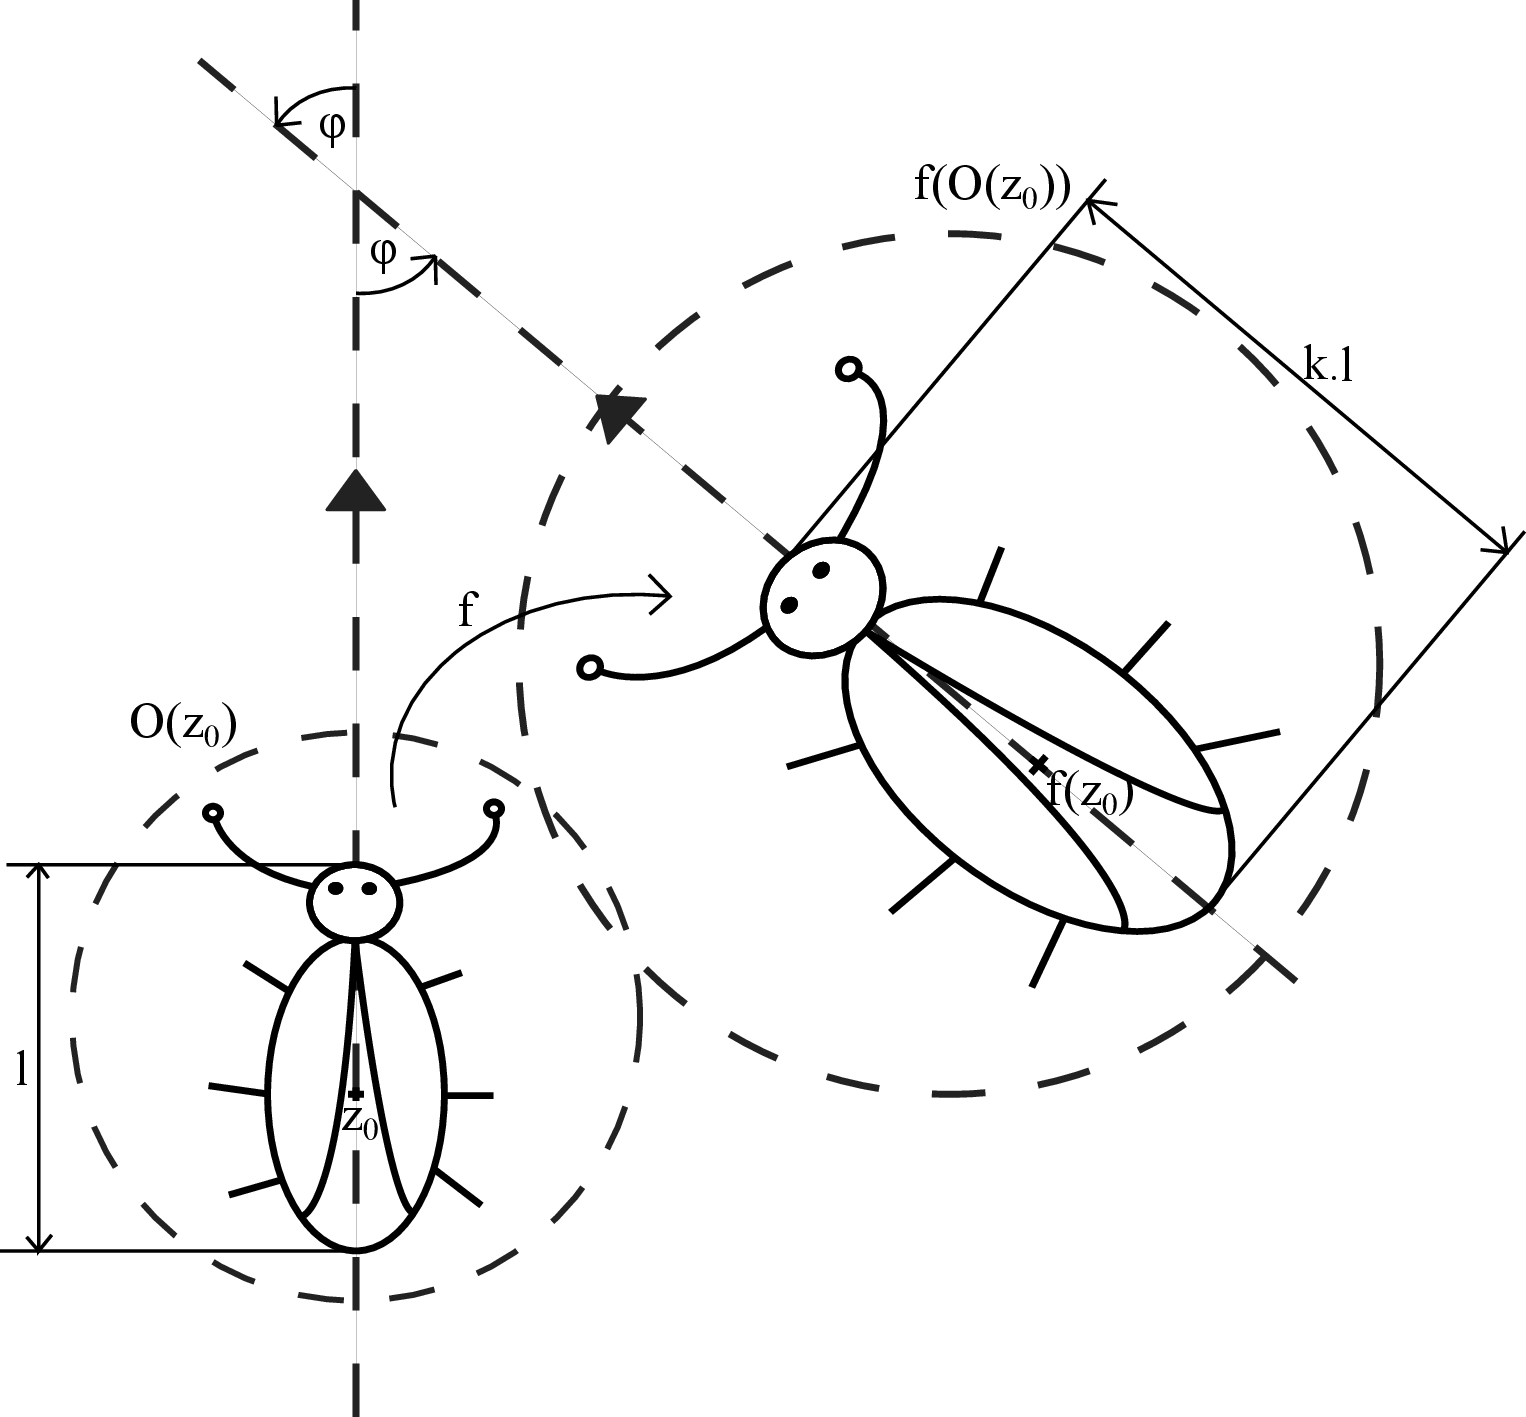
\includegraphics[scale=0.25]{Obrazky/Chroust.png}
\caption{Infinitezimální chroust}
\end{figure}


\section{Integrál v komplexním oboru}
\begin{definition}
	Mějme funkci $f(z)$, která má definiční obor $M \subseteq \mathbb{C}$. Nechť $\varphi(t), t \in \langle a,b \rangle$ je po částech hladká křivka taková, že její graf je podmnožina $M$ ($[\varphi] \subseteq M$). Pokud existuje $\int_a^b f(\varphi(t))\varphi'(t)\, \mathrm{d} t$, řekneme, že $f(z)$ je integrovatelná po křivce $\varphi$ a tento integrál značíme$\int_{\varphi} f(z)\, \mathrm{d} z$.
\end{definition}

\begin{definition}
	Nechť $\varphi(t), t \in \langle a,b \rangle$ je po částech hladká křivka. Délkou křivky nazýváme hodnotu integrálu $\int_a^b |\varphi'(t)|\, \mathrm{d} t$
 \end{definition}

\begin{definition}
(\textbf{Primitivní funkce)} Mějme funkci $f(z)$, která je definovaná na jednoduše souvislé oblasti $D \subseteq \mathbb{C}$. Řekneme, že funkce $F(z)$ je primitivní funkcí k $f(z)$, pokud $F'(z)=f(z), \forall z \in D$. Primitivních funkcí je nekonečně mnoho.
\end{definition}

\begin{theorem}
	Nechť \fce  $f(z)$ je holomorfní na $D$. Pak $\int_{\varphi}f(z) \, \dd z $ nezávisí na integrační cestě v $D$. Zapisujeme jej $\int_{z_1}^{z_2}f(z) \, \dd z = F(z_2)-F(z_1)$.
\end{theorem}

\begin{theorem}
	Následující 3 tvrzení jsou ekvivalentní na libovolné jednoduše souvislé oblasti $D \subseteq \mathbb{C}$
	\begin{itemize}
		\item Funkce $f(z)$ je holomorfní na $D$
		\item K funkci $f(z)$ existuje $F(z)$ na $D$
		\item $\int_{\varphi} f(z)\,  \dd z$ nezávisí na integrační cestě v $D$ 
	\end{itemize}
\end{theorem}

\begin{theorem}
\textbf{(Cauchyova věta- 1.verze)} Nechť $D \subseteq \mathbb{C} $ je jednoduše souvislá oblast a nechť $f(z)$ je funkce holomorfní na oblasti $D$ $\varphi$. Potom pro každou po částech hladkou Jordanova křivu takovou, že graf $[\varphi]\subset D $,  platí $\int_{\varphi} f(z)\, \dd z = 0.$
\end{theorem}



\begin{theorem}
\textbf{(Cauchyova věta- 2.verze)} Nechť $\varphi$ je po částech hladká Jordanova křivka a \fce $f(z)$ nechť je holomorfní na int$\varphi$ a je spojitá a ohraničená na $\overline{int\varphi}$. Pak platí, že $\int_{\varphi} f(z)\, \dd z=0.$  
\end{theorem}




%%%%%%%%%%%%%%%%%%%%%%%%%%%%%%%%%%%%%%%%%%%%%%%%%%%%%%%%%%%%%%
\textbf{Cauchyův integrální vzorec:}
Nechť $\varphi$ je po částech hladká kladně orientovaná Jordanova křivka. Nechť \fce\footnote{K výpočtu stačí znát funkcí jen na křivce $\varphi$} \fz je holomorfní na int$\varphi$, spojitá a ohraničená na $\overline{int\varphi}$. Potom platí $$f(z)=\frac{1}{2\pi 
i }\int_{\varphi}\frac{f(w)}{w-z}\, \dd w, \forall z \in \text{int}\varphi$$


\textbf{Cauchyův integrální vzorec pro n-tou derivaci:}
Nechť platí předpoklady předchozí věty. Potom platí:
$$f^{(n)}(z)=\frac{n!}{2\pi i}\int_{\varphi}\frac{f(w)}{(w-z)^{n+1}}\, \dd w, \forall z \in \text{int}\varphi$$

\begin{theorem}
	\textbf{(O jednoznačnosti holomorfní \fce)}
	Mějme \fce $f(z),g(z)$, které jsou holomorfní na oblasti $D \subset \CC$. Označme $M$ množinu všech bodů $z$, pro které platí $f(z)=g(z)$ tzn. $M=\{ z \in D | f(z)=g(z)\}$. Existuje-li v množině $M$ hromadný bod, pak pro každé $z\in D$ platí $f(z)=g(z)$.
	
\begin{dusledek}
	Zadám holomorfní funkci na reálné ose, libovolném kousku Gauss. roviny s nenulovou plochou, grafu libovolné křivky $\Rightarrow$ \fce je zadána v celém $\CC$.
\end{dusledek}
\end{theorem}

\begin{definition}
	\textbf{Rezidua}
	Nechť \fce \fz je holomorfní v nějakém okolí $O(z_0)$ bodu $z_0 \in \overline{\CC}$  s případnou výjimkou bodu $z_0$.
    \begin{itemize}
    \item Nechť $z_0 \in \CC$. Nechť   $\sum_{n=-\infty}^{\infty}a_n(z-z_0)^n$ je Laurentova řada funkce \fz, která konverguje k funkci \fz na množině $O(z_0)\setminus \{z_0\}$. Reziduem funkce \fz v bodě $z_0$ nazveme koeficient $a_{-1}$ Laurentovy řady a zavedem označení $\mathrm{Res}_{z=0} f(z)=a_{-1}$  
\item  Nechť $z_0=\infty$. Nechť  $\sum_{-\infty}^{\infty} a_nz^n$ je Laurentova řada funkce \fz se středem v bodě $\infty $, která kon verguje k funkci \fz na množině $O(\infty)\setminus \{\infty\}$. Reziduem funkce \fz v bodě $\infty $ nazveme koeficient $-a_{-1}$ Laurentovy řady a zavedeme označení $Res_{z=\infty} \, f(z)=-a_{-1}$.
    \end{itemize}
\end{definition}

\begin{theorem}
Nechť $z_0\in \CC$ a nechť funkce \fz je holomorfní na nějakém okolí $O(z_0)$ bodu $z_0$ s případnou výjimkou bodu $z_0$. Pak platí 
\begin{equation*}
\mathrm{Res}_{z=z_0}f(z)=\frac{1}{2\pi i}\int_{\varphi_{\rho}}f(z) \, \mathrm{d} z,
\end{equation*}
 kde $\varphi_{rho}(t)=z_0+\rho\mathrm{e}^{it}, t \in \langle 0,2\pi \rangle$ a $\rho$ je voleno tak, aby $[\varphi_{\rho}] \subset O(z_0) \setminus \{z_0\}$.
 
 A nechť  $z_0=\infty $ a nechť funkce \fz je holomorfní na nějakém okolí $O(\infty)$ bodu $\infty$ s případnou výjimkou bodu $\infty$. Pak platí 
\begin{equation*}
\mathrm{Res}_{z=\infty}f(z)=-\frac{1}{2\pi i}\int_{\varphi_{\rho}}f(z) \, \mathrm{d} z,
\end{equation*}
 kde $\varphi_{rho}(t)=\rho\mathrm{e}^{it}, t \in \langle 0,2\pi \rangle$ a $\rho$ je voleno tak, aby $[\varphi_{\rho}] \subset O(\infty) \setminus \{\infty\}$.
 \end{theorem}

\begin{theorem}
	Nechť \fce \fz má v bodě $z_0 \in \CC$ pól řádu $k$, tak platí, že 
	$$Res_{z=z_0} \, f(z)=\frac{1 }{(k-1)!} \lim_{z\rightarrow z_0}[(z-z_0)^k \, f(z)]^{(k-1)}$$
\end{theorem}
\begin{theorem}
	Nechť \fce \fz má v bodě $\infty$ pól řádu $k$, kde $k \geq -1$, potom platí, že 
	$$Res_{z=\infty} f(z) = \frac{(-1)^k}{(k+1)!} \lim_{z \rightarrow \infty} z ^{k+2}f(z)^{(k+1)}$$
	Pokud $k<-1$, pak $Res_{z=\infty}(f)=0$
\end{theorem}
%%%%%%%%%%%%%%%%%%%%%%%%%%%%%%%%%%%%%%%%%%%%%%%%%%%%%%%%%%%%%%


%%%%%%%%%%%%%%%%%%%%%%%%%%%%%%%%%%%%%%%%%%%%%%%%%%%%%%%%%%%%%%
\begin{theorem}
	Nechť \fce \fz je holomorfní v celém $\CC$ s výjimkou konečného počtu singulárních bodů $z_1,z_2,\ldots, z_n. $ Označme $z_{n+1}=\infty$, pak platí  $\sum_{k=1}^{n+1}\text{Res}_{z=z_k}\, f(z)=0$.  
\end{theorem}

\begin{theorem}
\textbf{(Reziduální věta I)}
Nechť \fce \fz je holomorfní na jednoduše souvislé oblasti $D \subseteq \CC $ s výjimkou konečného počtu singulárních bodů $z_1,z_2,\ldots, z_k \in D.$ Nechť $\varphi$ je po částech hladká kladně orientovaná Jordanova křivka taková, že $[\varphi] \subseteq D $ a její graf neprochází žádným singulárním bodem. Označme $z_1,z_2,\ldots z_n$ všechny singulární body ležící v int$\varphi$. Pak platí, že $\int_{\varphi} f(z) \,  \dd z= 2\pi i\sum_{l=1}^{n}Res_{z=z_l} f(z)  $ 

%%%%%%%%%%%%%%%%%%%%%%%%%%%%%%%%%%%%%%%%%%%%%%%%%%%%%%%%	
\end{theorem}

\begin{theorem}
\textbf{(Reziduální věta II)}
Nechť \fce \fz je holomorfní v $\CC$ s výjimkou konečného počtu singulárních bodů $z_1,z_2,\ldots, z_k$. Nechť $\varphi$ je po částech hladká, kladně orientovaná Jordanova křivka taková, že $[\varphi]$ neprochází žádným singulárním bodem. Označme $z_1,z_2,\ldots, z_n$ všechny singulární body ležící v ext$\varphi$ a označme $z_{n+1}=\infty$. Poté platí, že $\int_{\varphi} f(z) \, \dd z = -2\pi i \sum_{l=1}^{n+1}Res_{z=z_l} f(z)$
\end{theorem}

%\begin{figure}[H]
%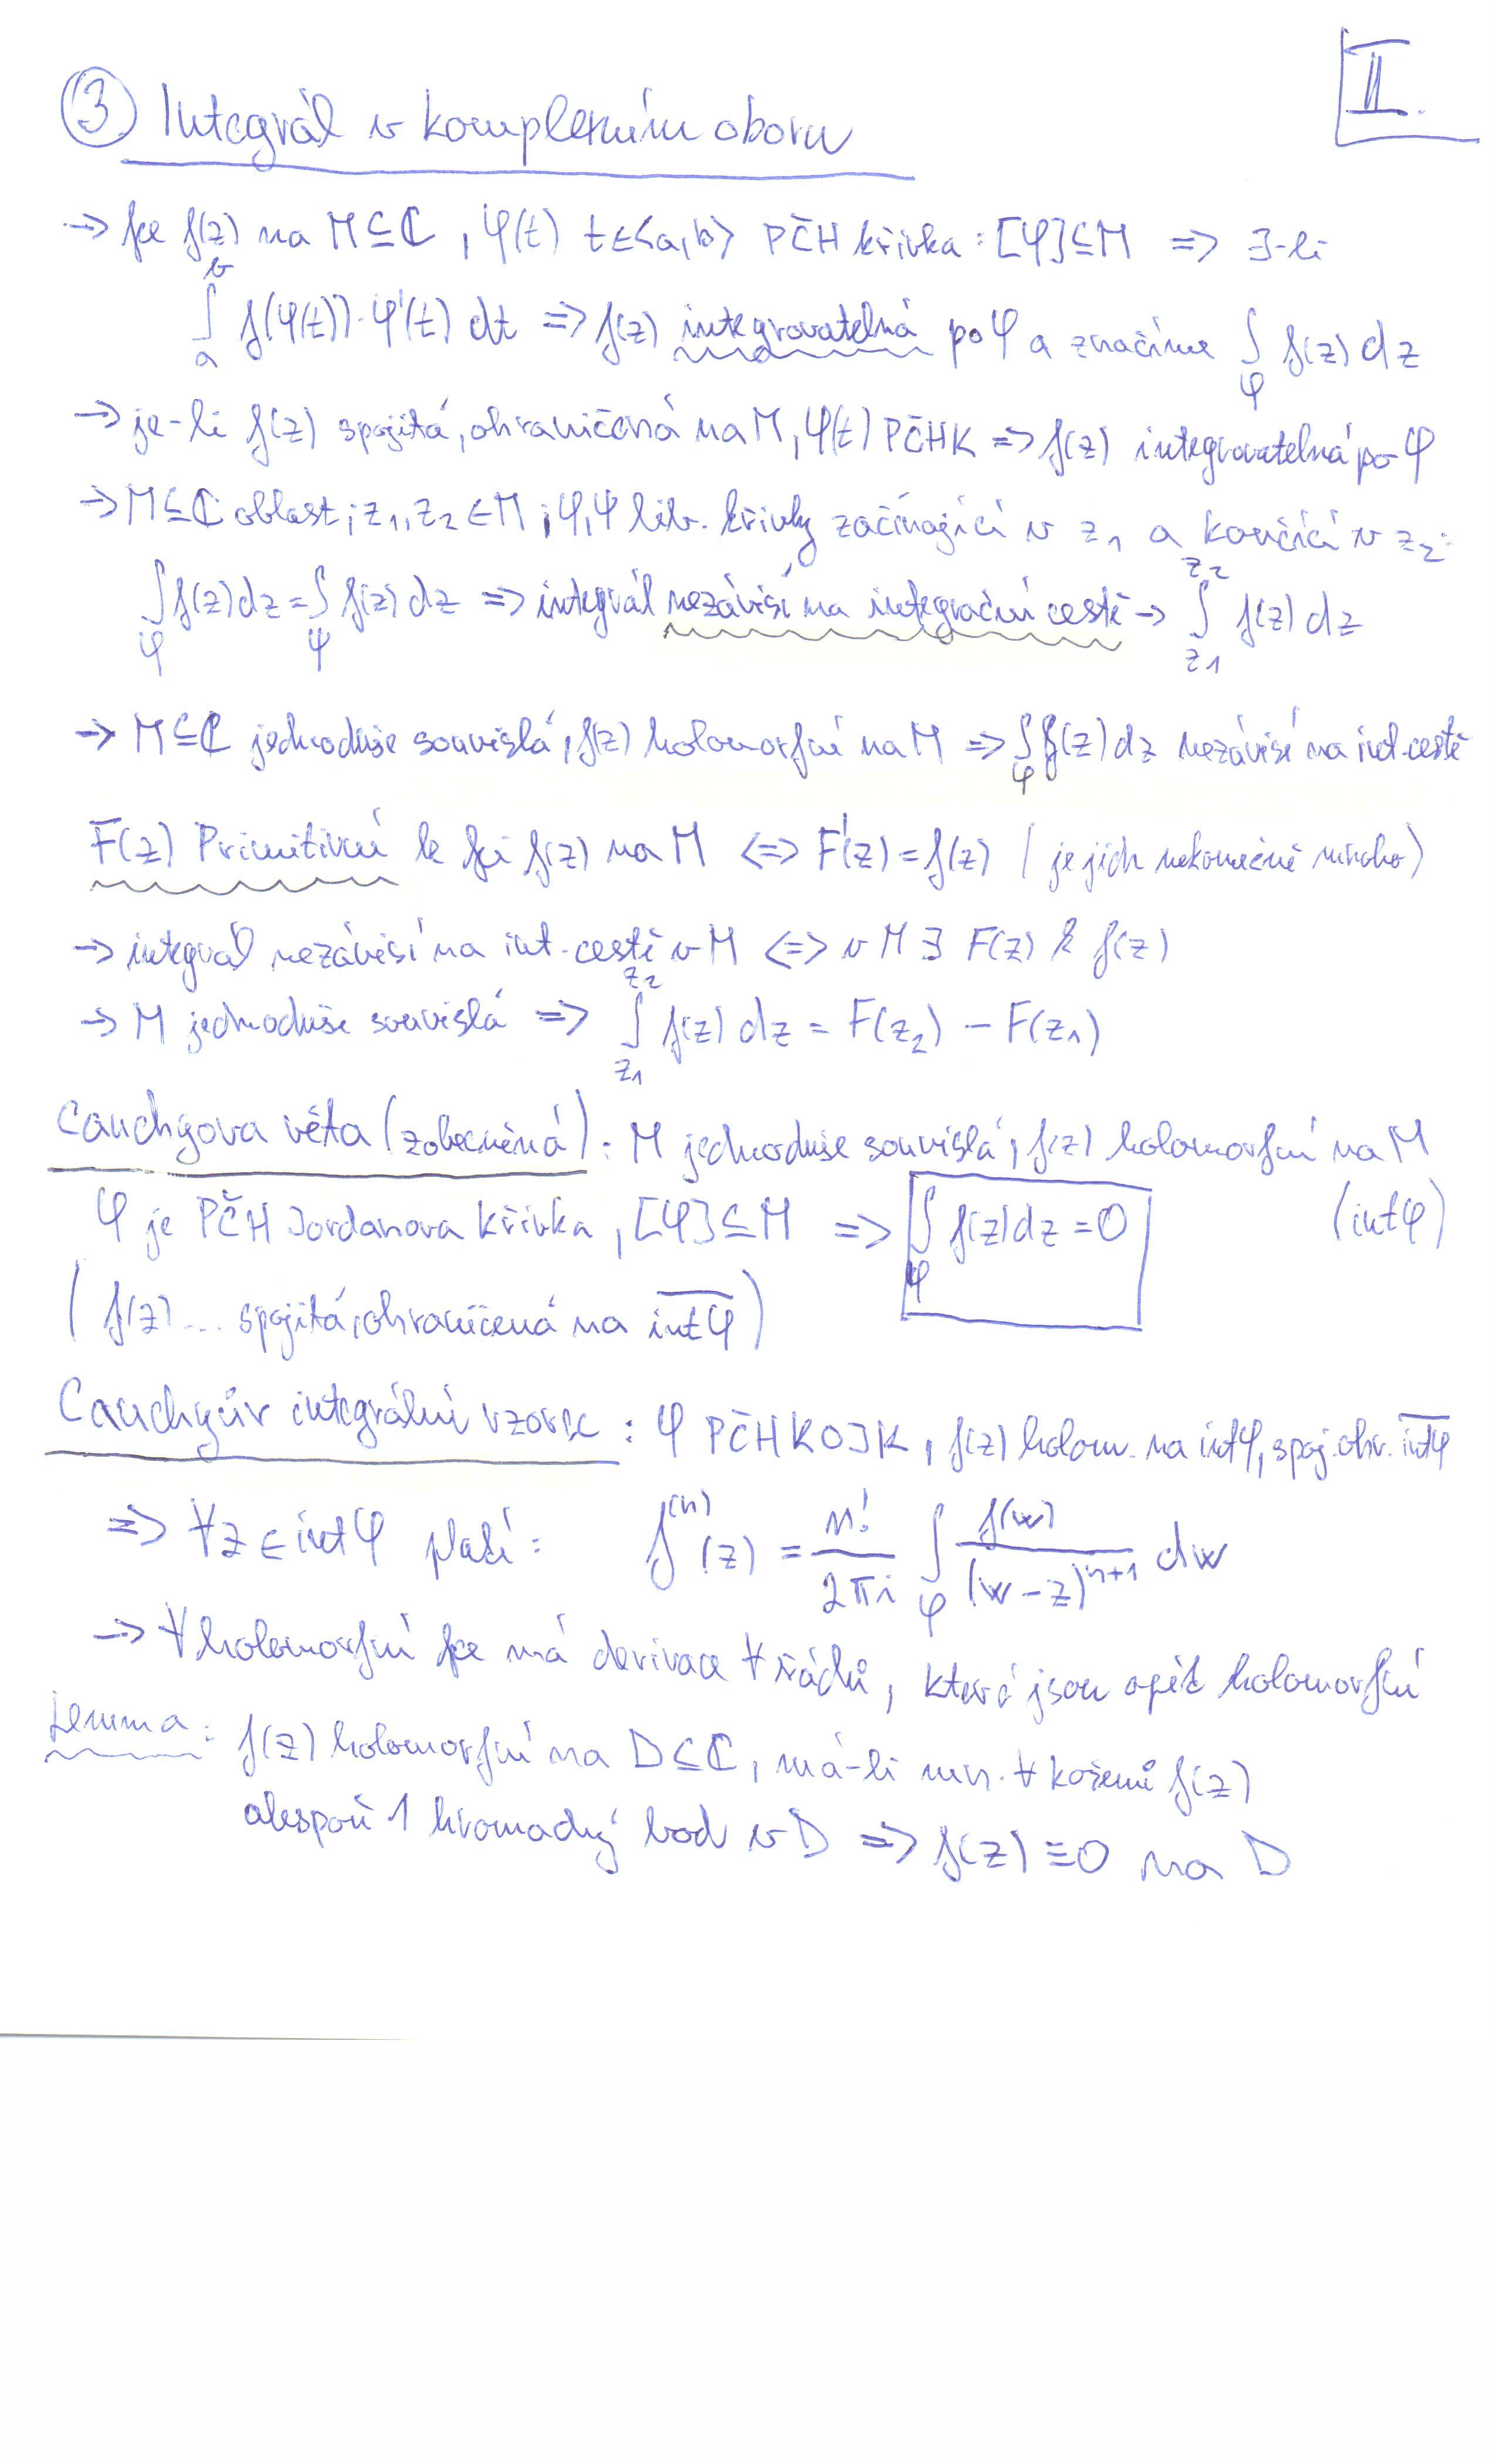
\includegraphics[width=\textwidth]{2-3a.jpg}
%\end{figure}

%\begin{figure}[H]
%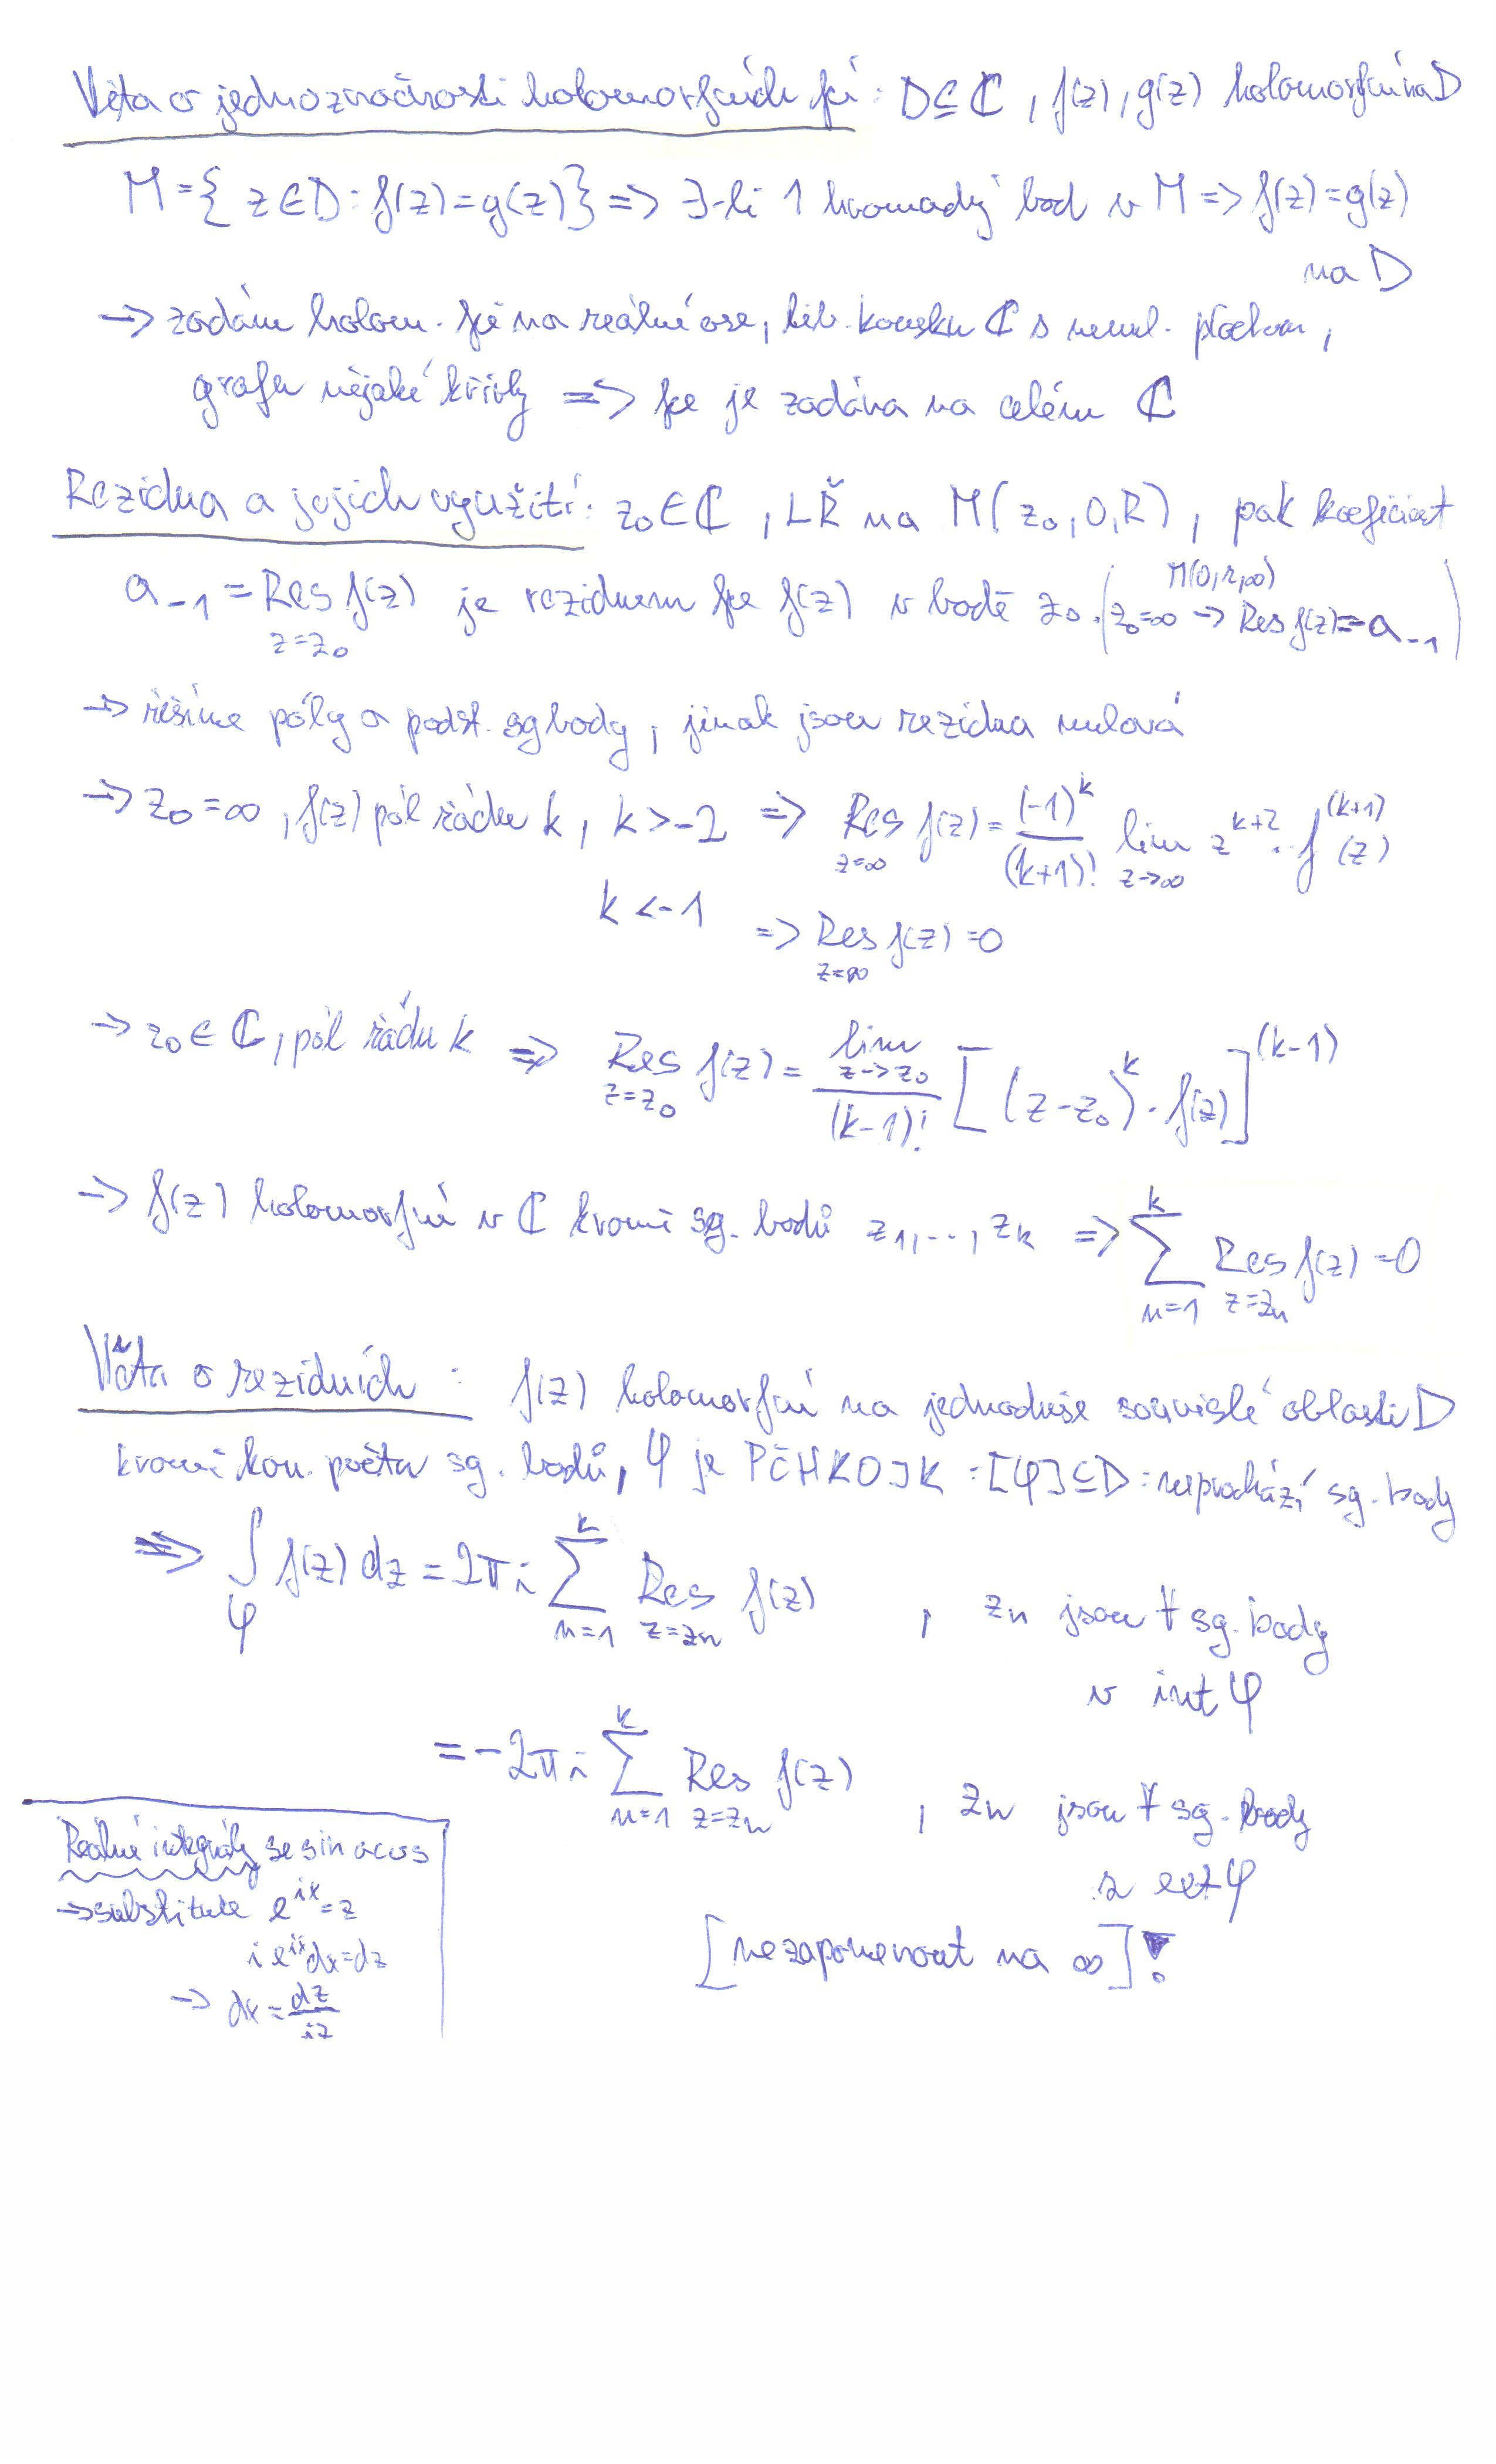
\includegraphics[width=\textwidth]{2-3b.jpg}
%\end{figure}


\section{Konformní zobrazení}
\subsection{Konformní zobrazení: věta o zachování úhlů, konformní ekvivalentnost oblastí, Riemannova věta}
\begin{definition}
	Nechť $M,N$ jsou otevřené množiny. Nechť $f:M\rightarrow N$ má následující vlastnosti:
	\begin{itemize}
		\item \fz je bijekce
		\item \fz je holomorfní
		\item $f'(z)\neq 0$ pro $\forall z \in M$
	\end{itemize}
\end{definition} 
Pak řekneme, že \fz je konformním zobrazením množiny $M$ na množinu $N$.

\begin{theorem}
	Nechť $\varphi$ a $\psi$ jsou dvě hladké křivky takové, že průnik jejich grafů $[\varphi] \cap [\psi]=\{z_0\}, z_0\in \CC $ a $z_0$ není počáteční, ani koncový bod grafů.
	Nechť $p$ je orientovaná tečna ke grafu $[\varphi]$ v bodě $z_0$ a $q$ je orientovaná tečna ke grafu $[\psi]$ v bodě $z_0$. Nechť \fz je holomorfní na okolí $O(z_0)$. Nechť $t$ je orientovaná tečna ke grafu $[f(\varphi)]$ v bodě $f(z_0)$ a s je orientovaná tečna ke grafu $[f(\psi)]$ v bodě $f(z_0).$ Nechť $f'(z_0) \neq 0$. Pak platí, že orientovaný úhel $\sphericalangle (p,q)=\sphericalangle (t,s)$   
\end{theorem}
%%%%%%%%%%%%%%%%%%%%%%%%%%%%%%%%%%%%%%%%%%%%%%%%%%%%%%%%%%%%%%

%%%%%%%%%%%%%%%%%%%%%%%%%%%%%%%%%%%%%%%%%%%%%%%%%%%%%%%%%%%%%%
\begin{definition}
	Řekneme, že dvě otevřené množiny $M,N \subseteq \CC$ jsou konformně ekvivalentní $(M\sim_K N)$, existuje-li mezi nimi konformní zobrazení.
\end{definition}

\begin{theorem}
	Nechť $M,N, K \subseteq \CC$ jsou otevřené množiny potom platí
	\begin{itemize}
		\item $f(z)=z$ je konformní zobrazení $M$ na $M$
		\item Je-li $f:M\rightarrow N$ konformní zobrazení, pak $f^{-1}: N\rightarrow M$ je konformní zobrazení $N$ na $M$.
		\item $f:M\rightarrow N$ je konformní zobrazení a $g:N\rightarrow K$ je konformní zobrazení $N$ na $K$, pak funkce $g \circ f:M\rightarrow K$ je konformní zobrazení $M$ na $K$.
	\end{itemize}
\end{theorem}

\begin{theorem}
	\textbf{Riemannova věta:} Nechť $M,N$ jsou dvě jednoduše souvislé oblasti, které jsou vlastními podmnožinami $\CC, (M,N \subset \CC) $ pak $N\sim_K M$
\end{theorem}

\begin{theorem}
	Neexistuje jiná množina od $\CC$ pro kterou platí $M\sim_K \CC$, tj. $\CC $ není konformně ekvivalentní s~žádnou vlastní podmnožinou.
\end{theorem}

\begin{theorem}
	Nechť $M\subseteq \CC$ je k-násobně souvislá oblast. Nechť $N \subseteq \CC $ je l-násobně souvislá oblast a nechť platí, že $M\sim_K N$. Pak $k=l$.
\end{theorem}


%\begin{figure}[H]
%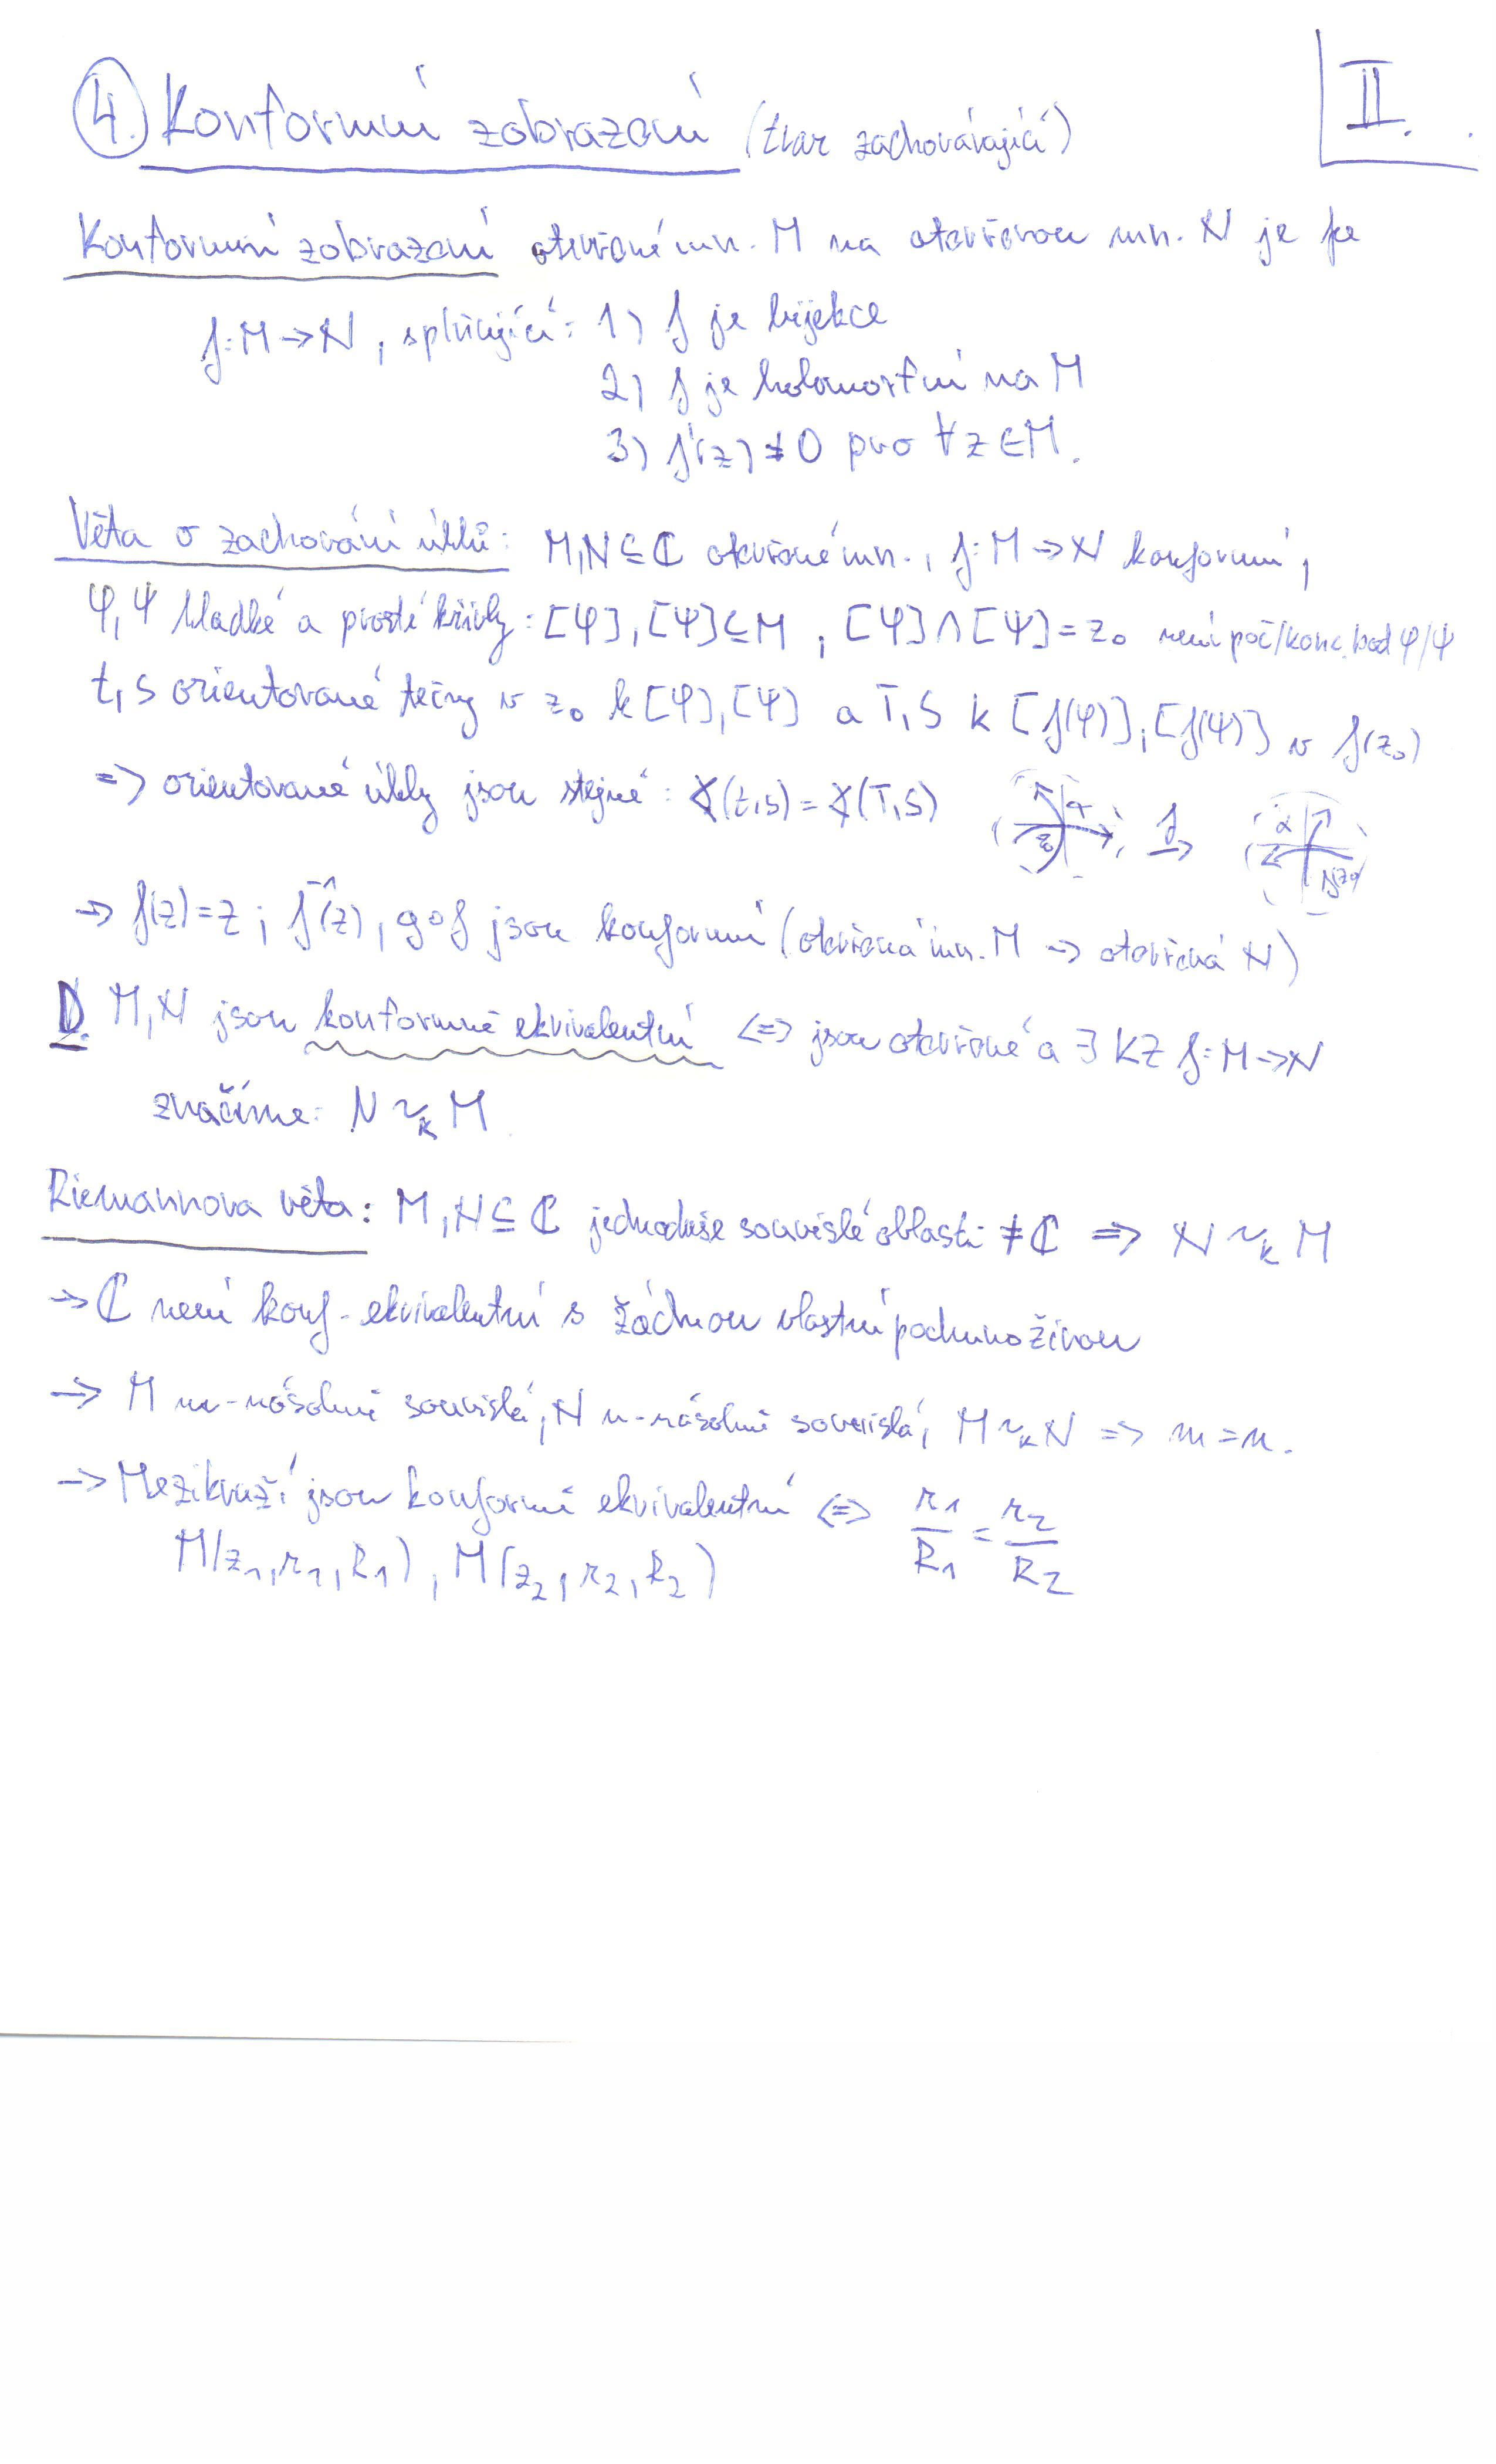
\includegraphics[width=\textwidth]{2-4a.jpg}
%\end{figure}

%\begin{figure}[H]
%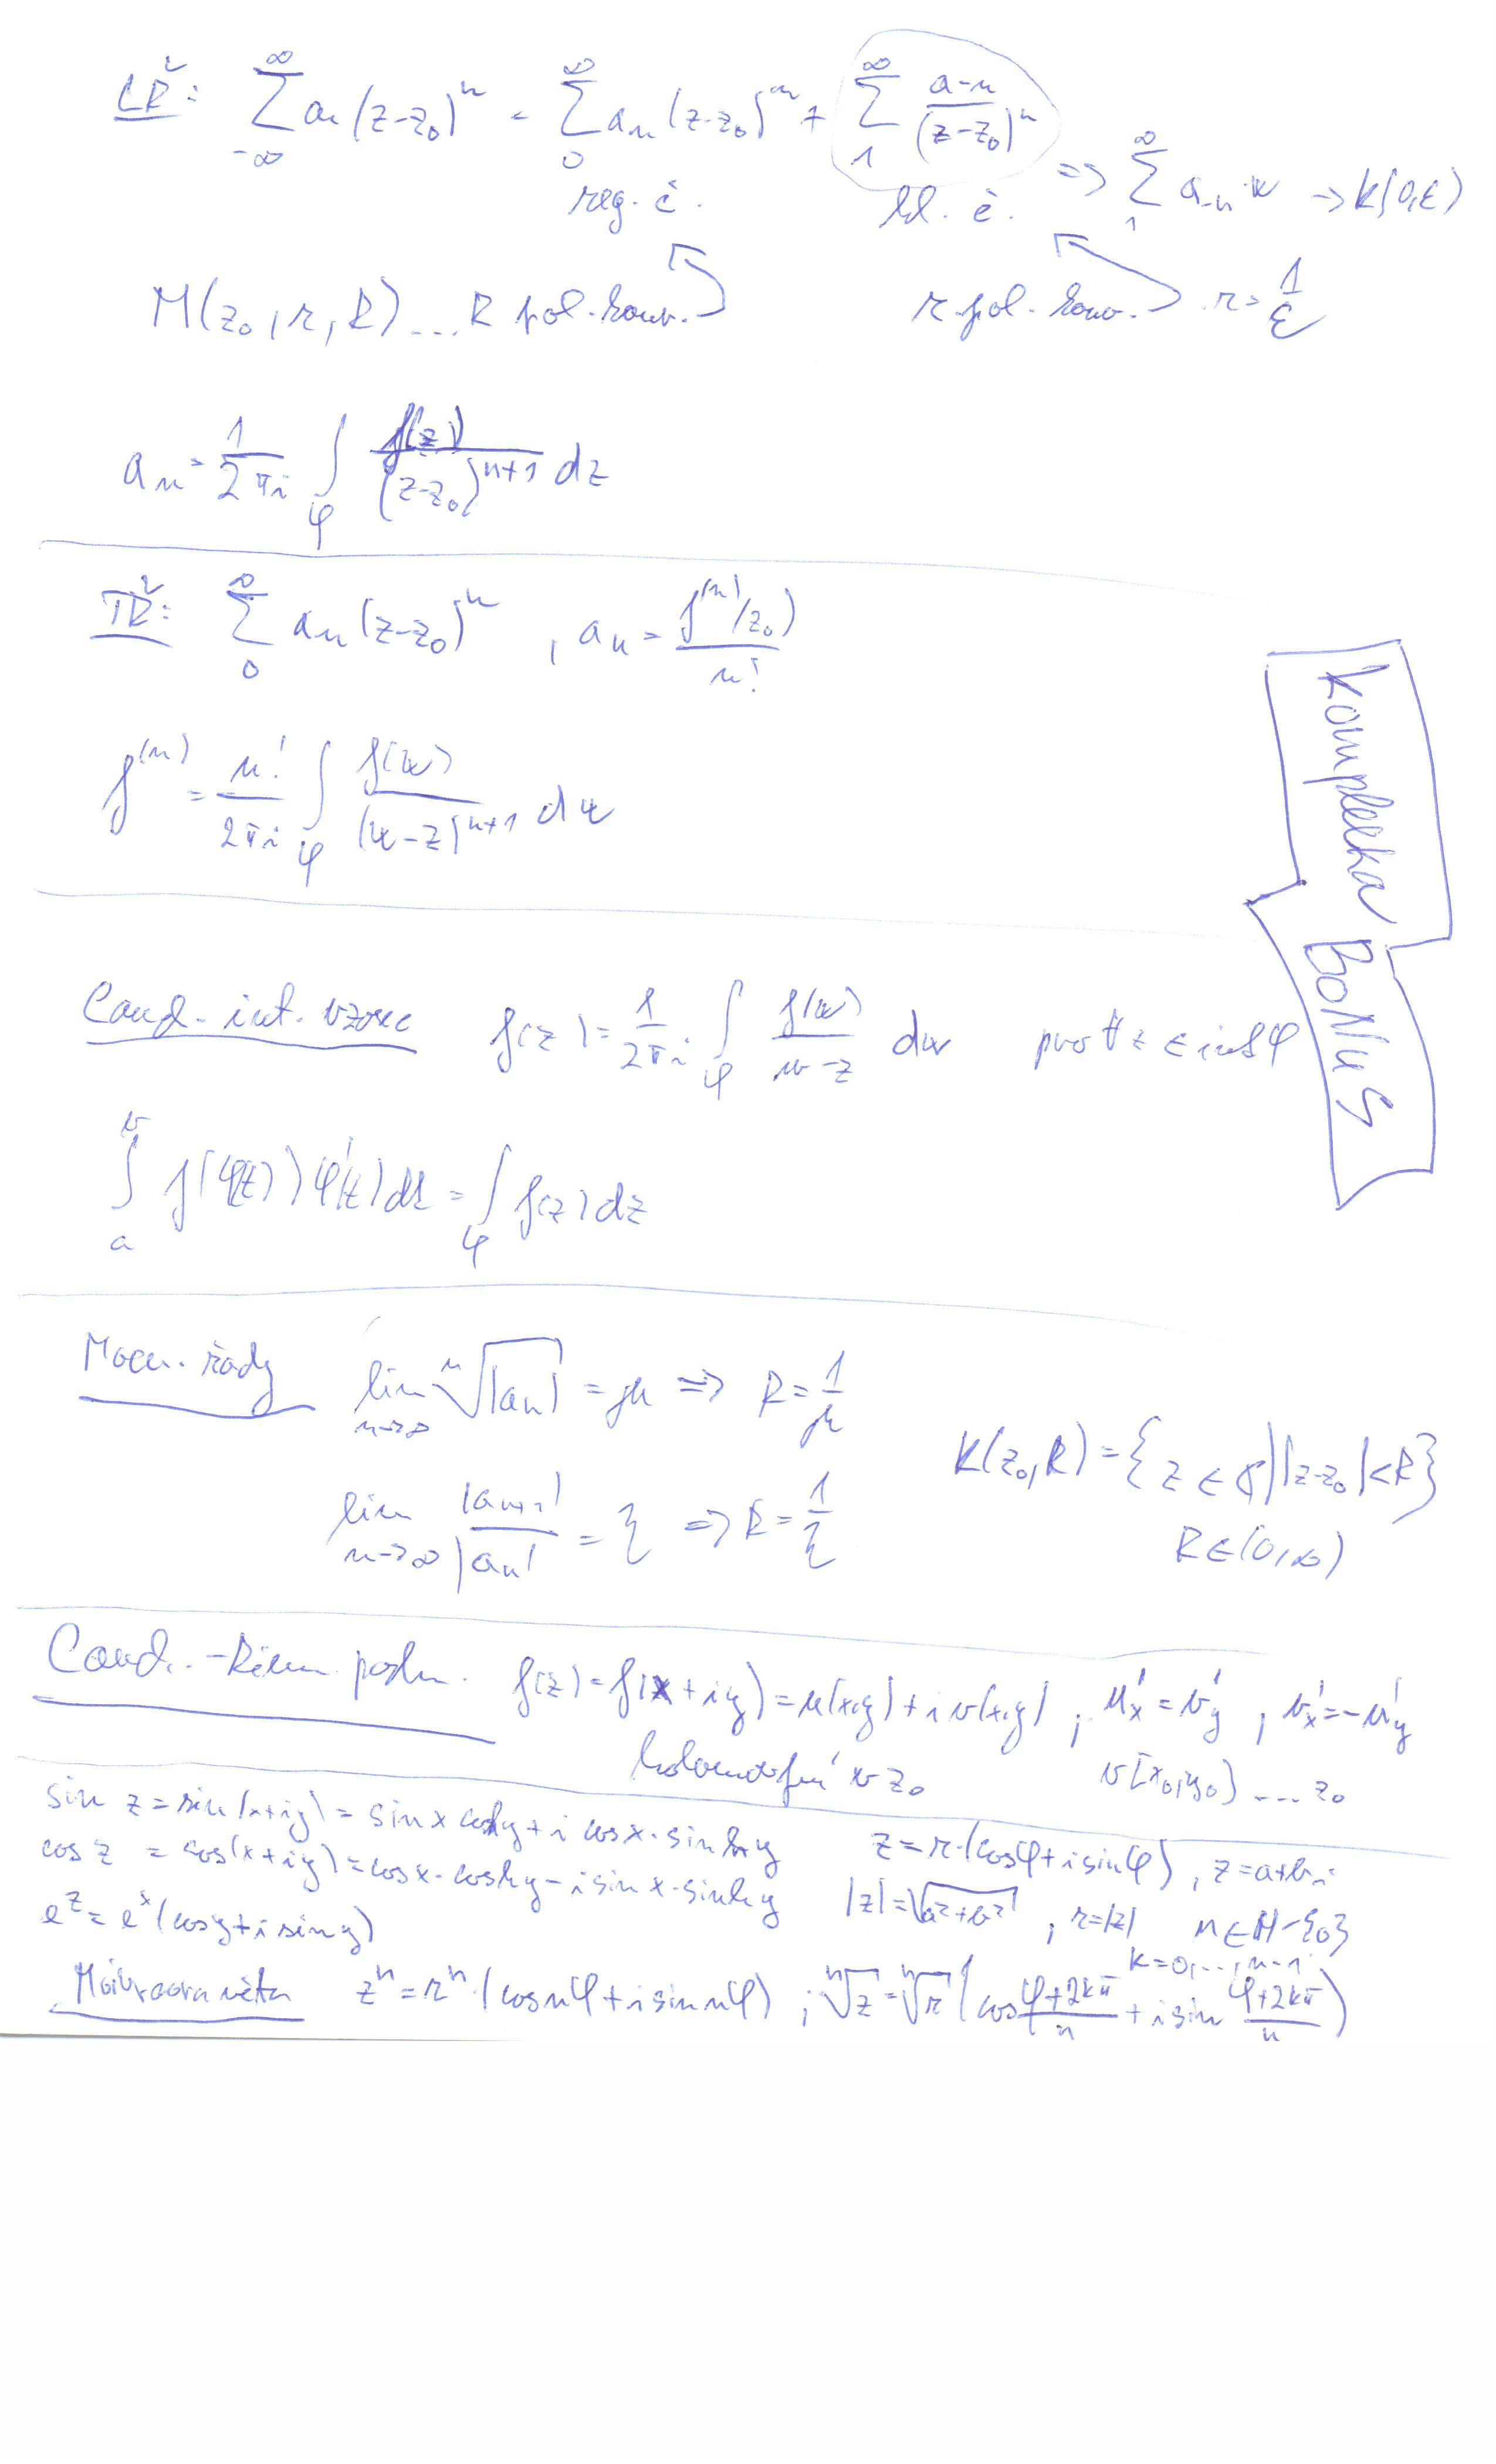
\includegraphics[width=\textwidth]{2-4b.jpg}
%\end{figure}

\begin{figure}[H]
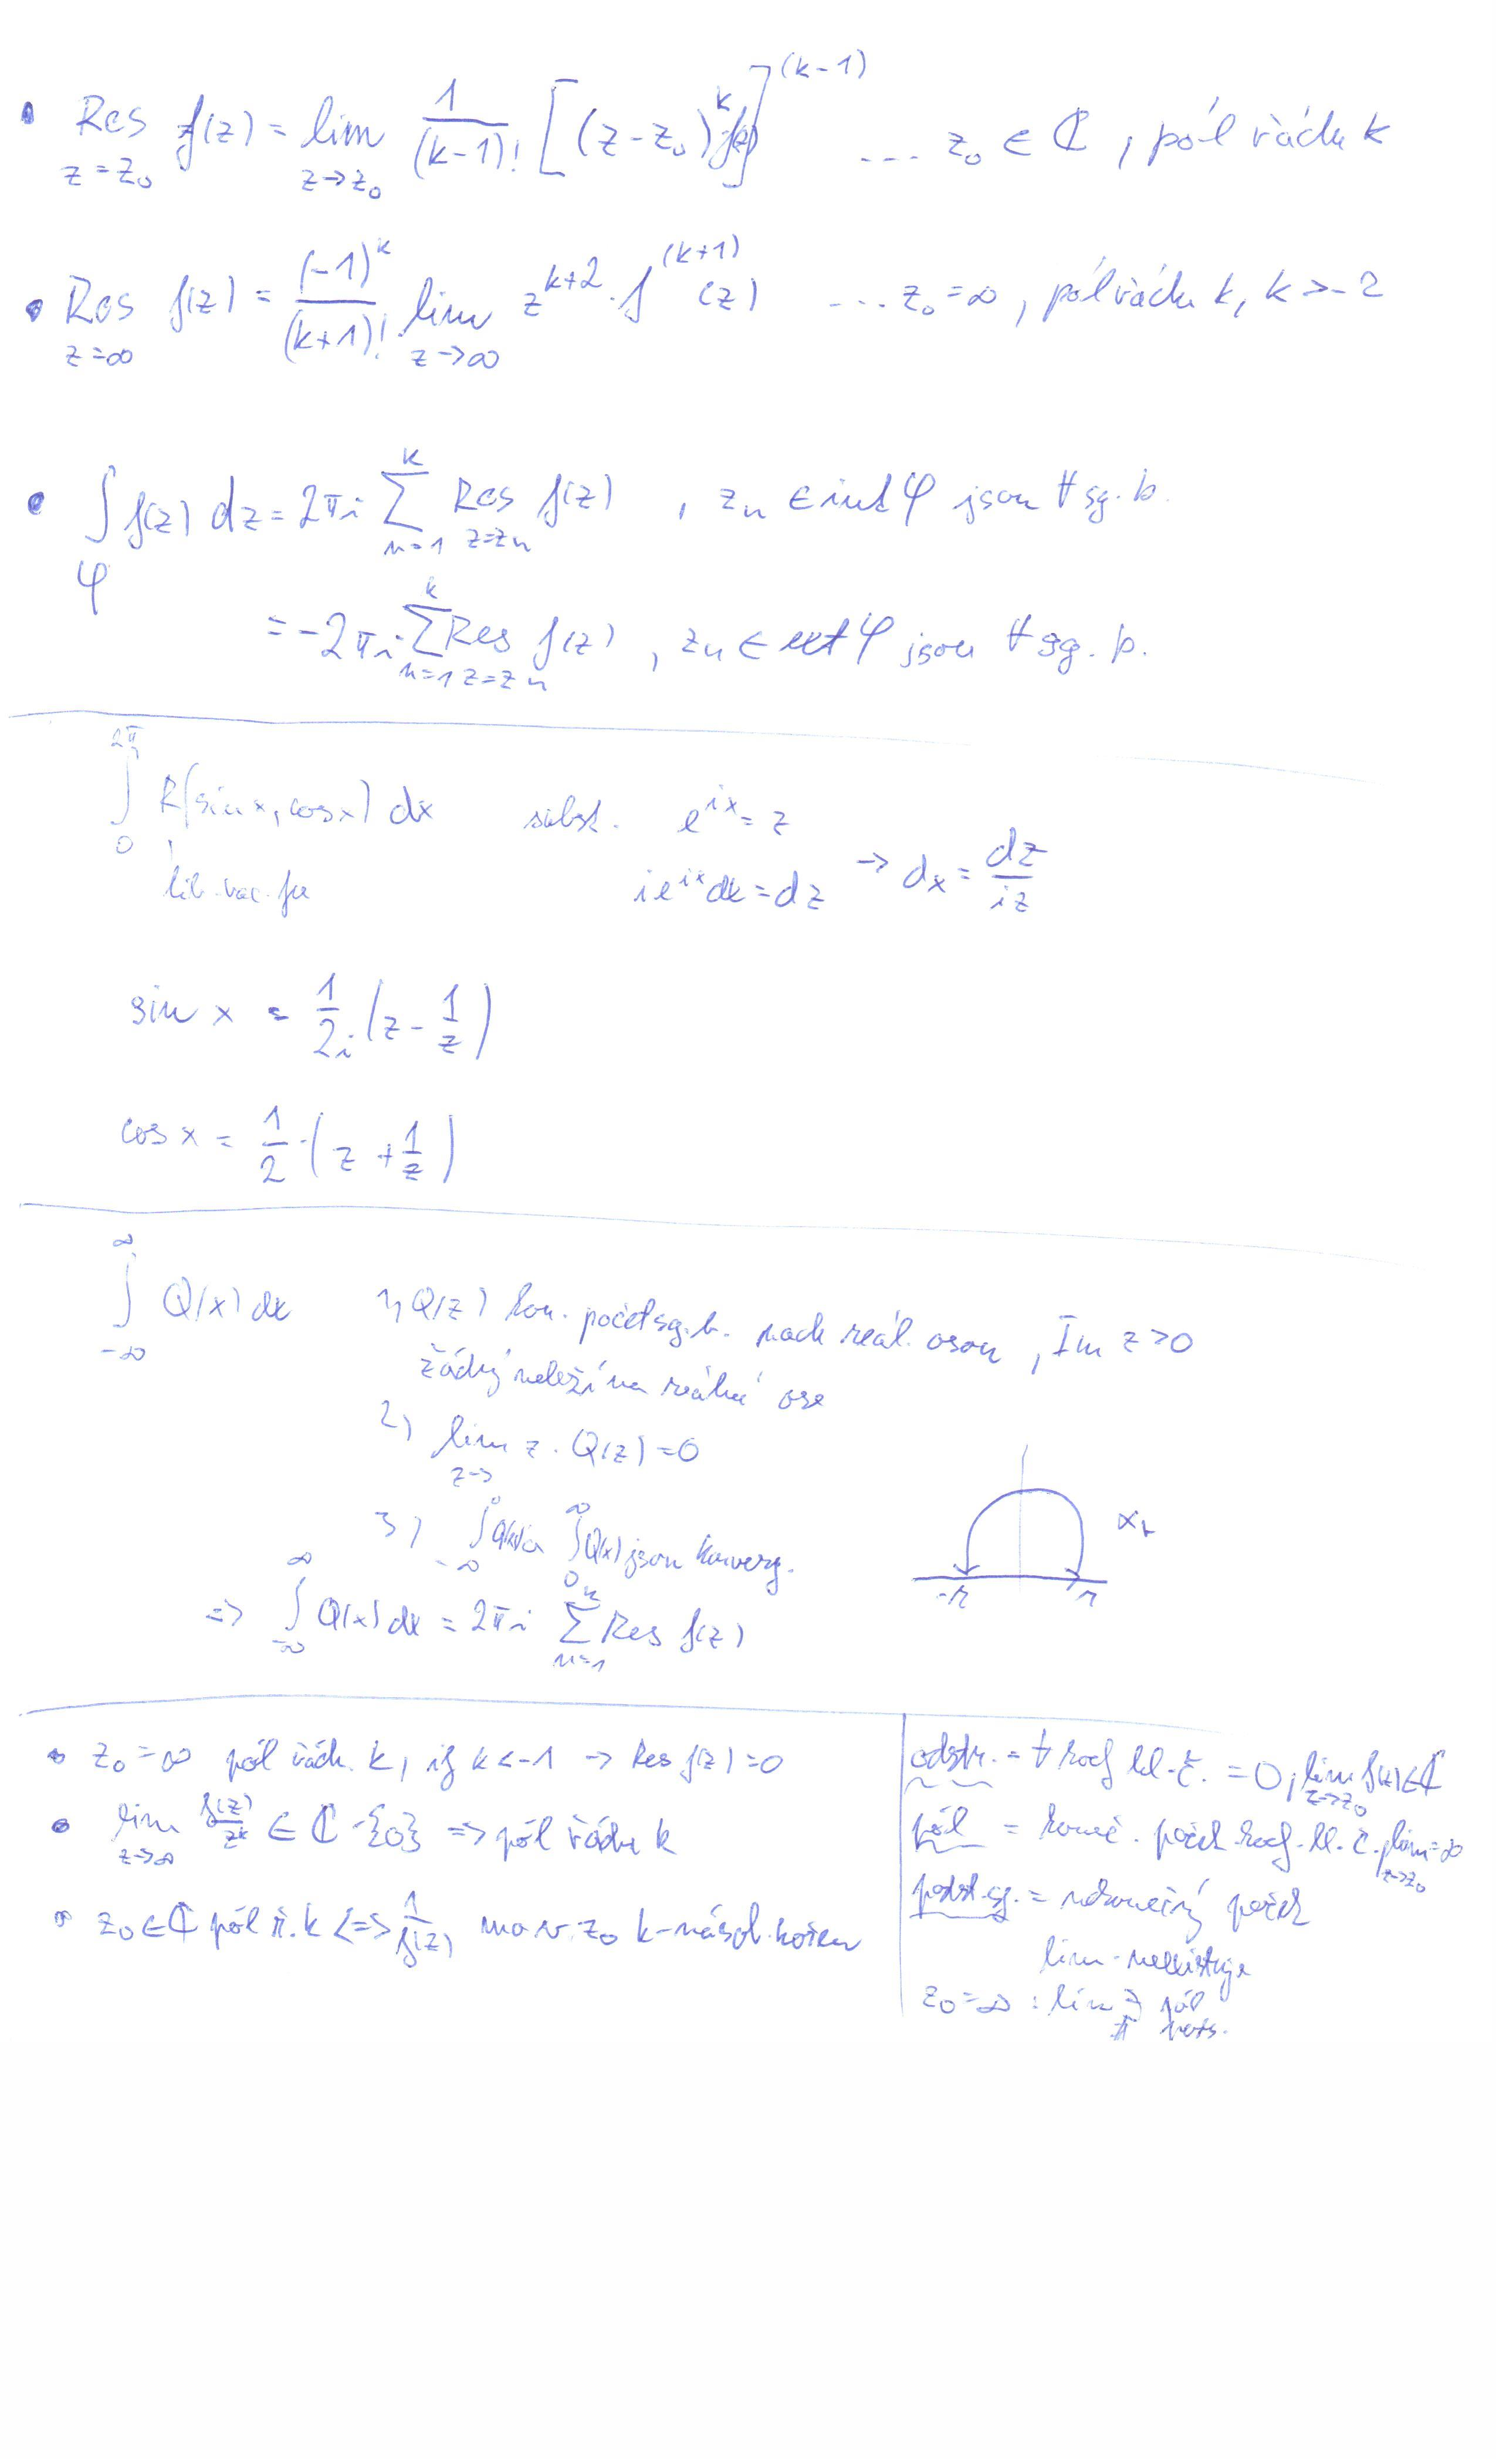
\includegraphics[width=\textwidth]{Obrazky/2-4c.jpg}
\end{figure}

\begin{figure}[H]
\section{Klasická teorie PDR}
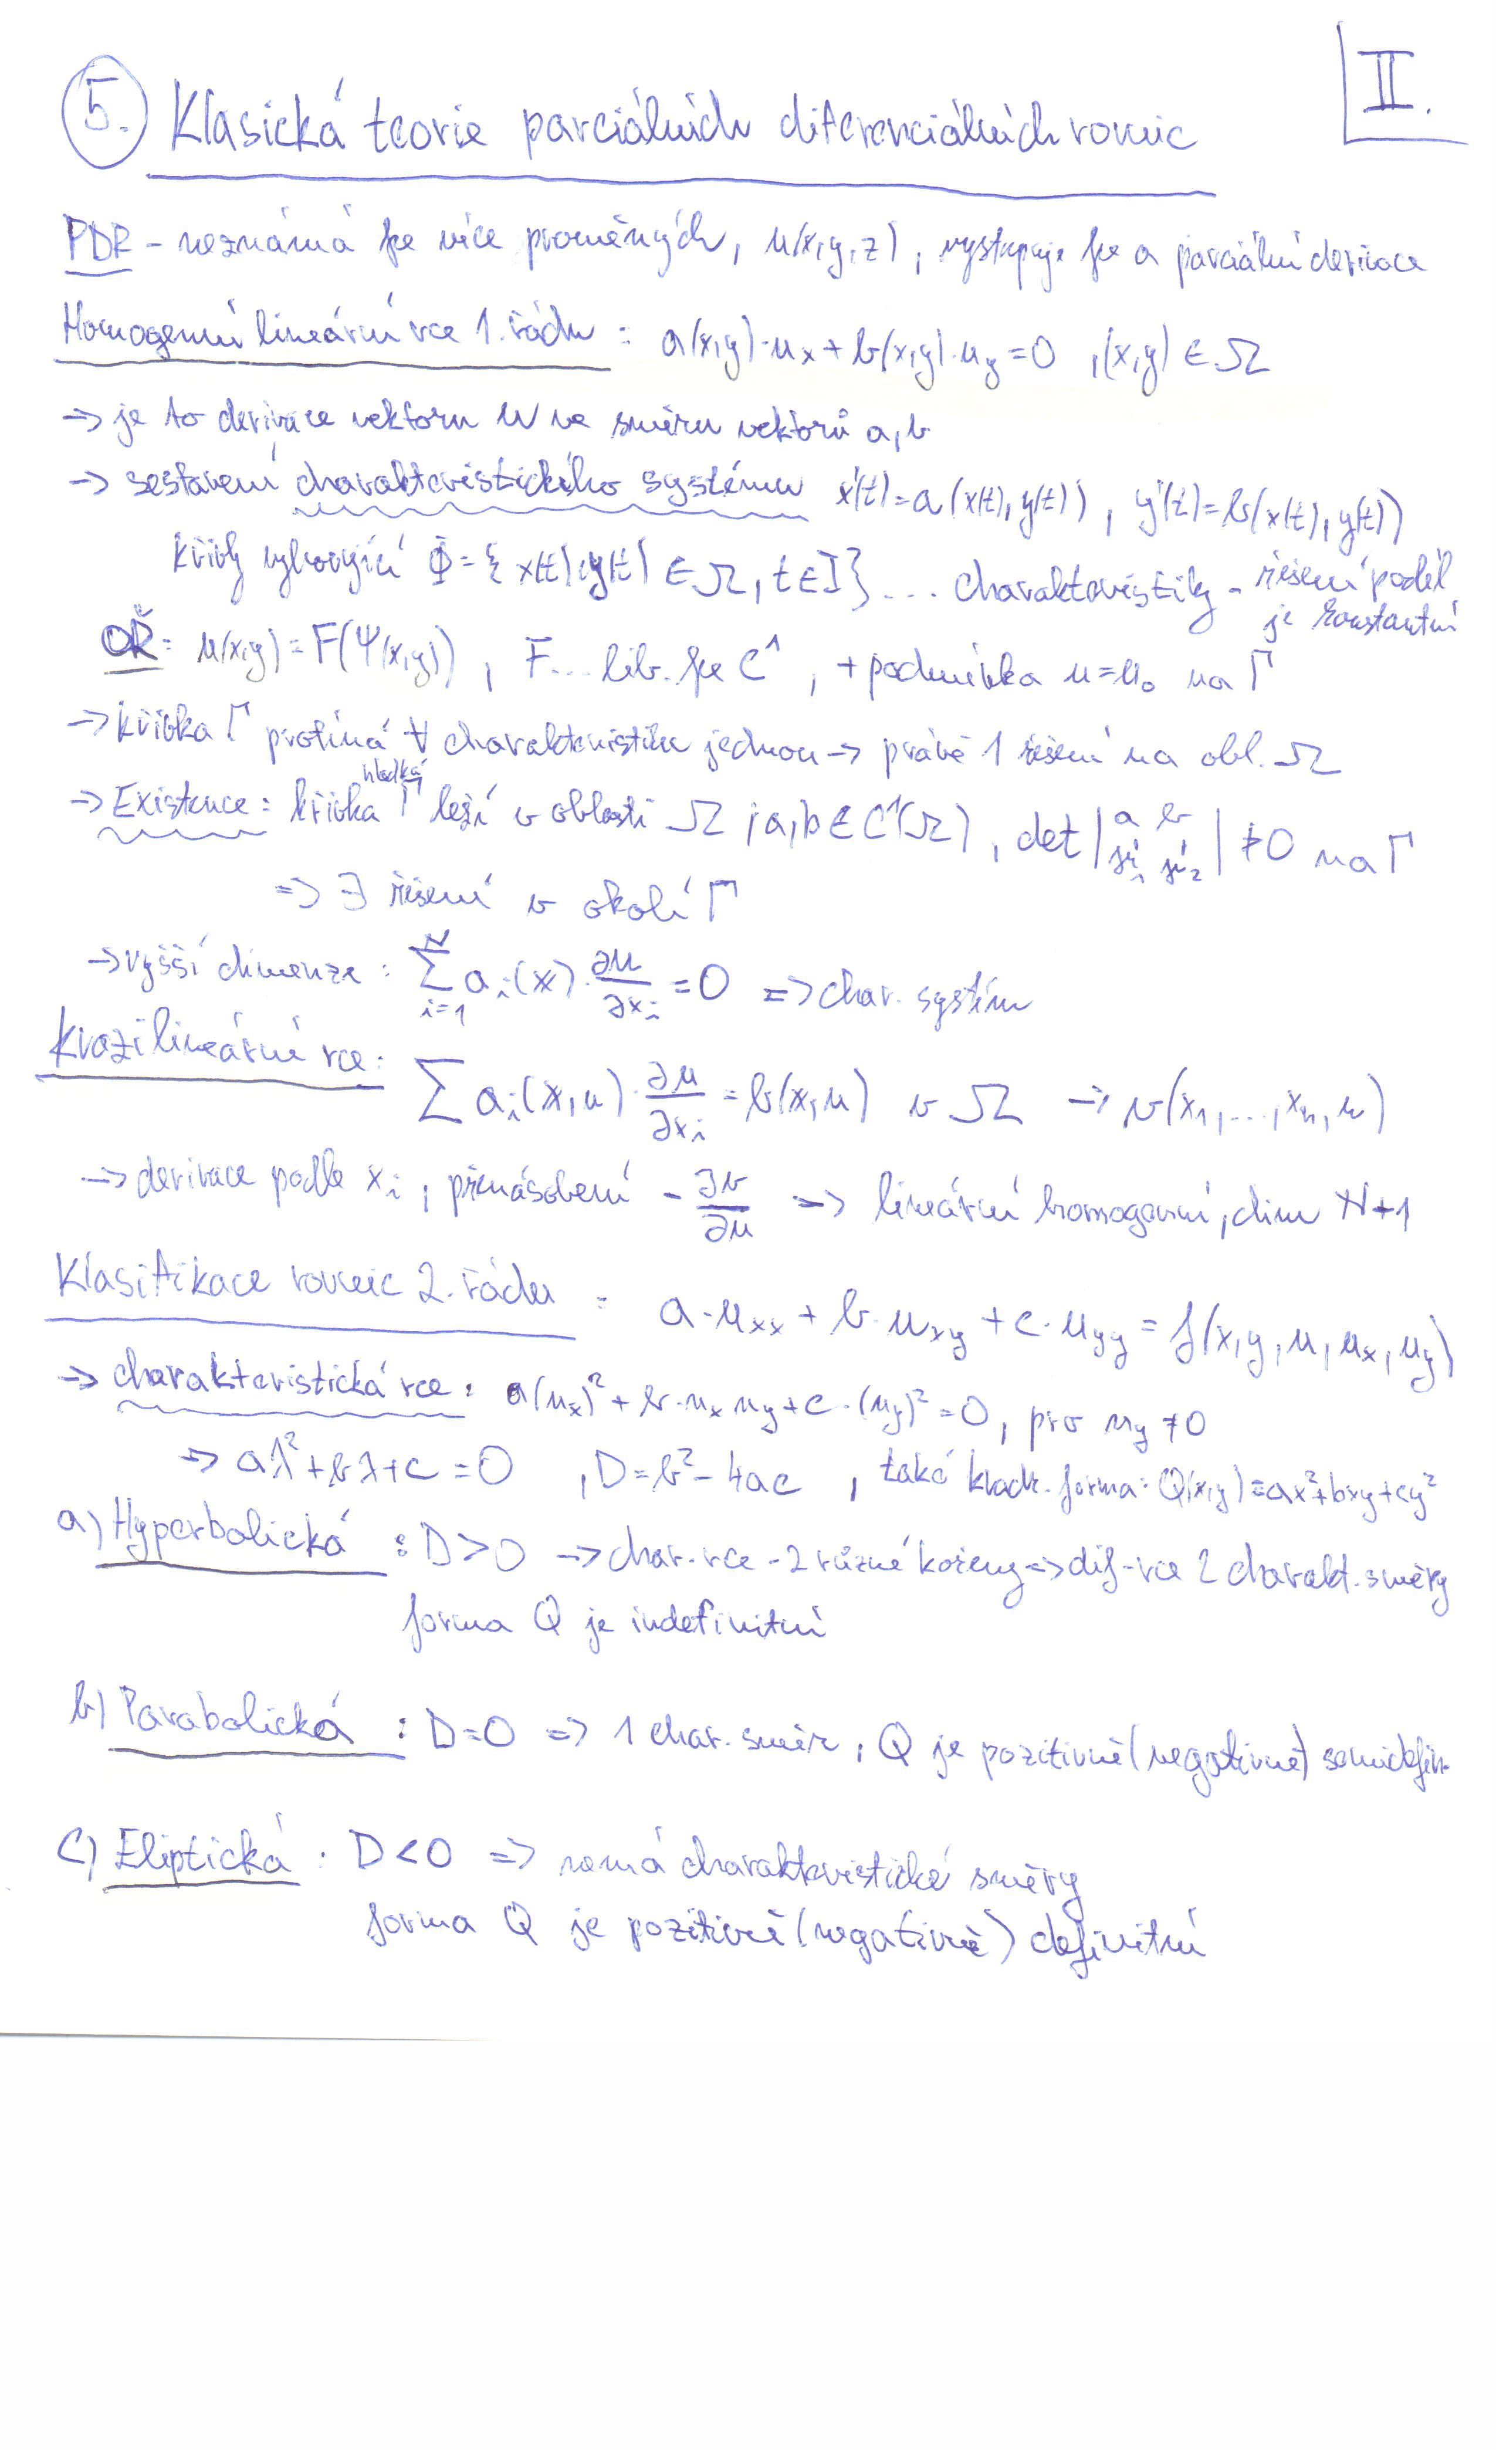
\includegraphics[width=\textwidth]{Obrazky/2-5a.jpg}
\end{figure}

\begin{figure}[H]
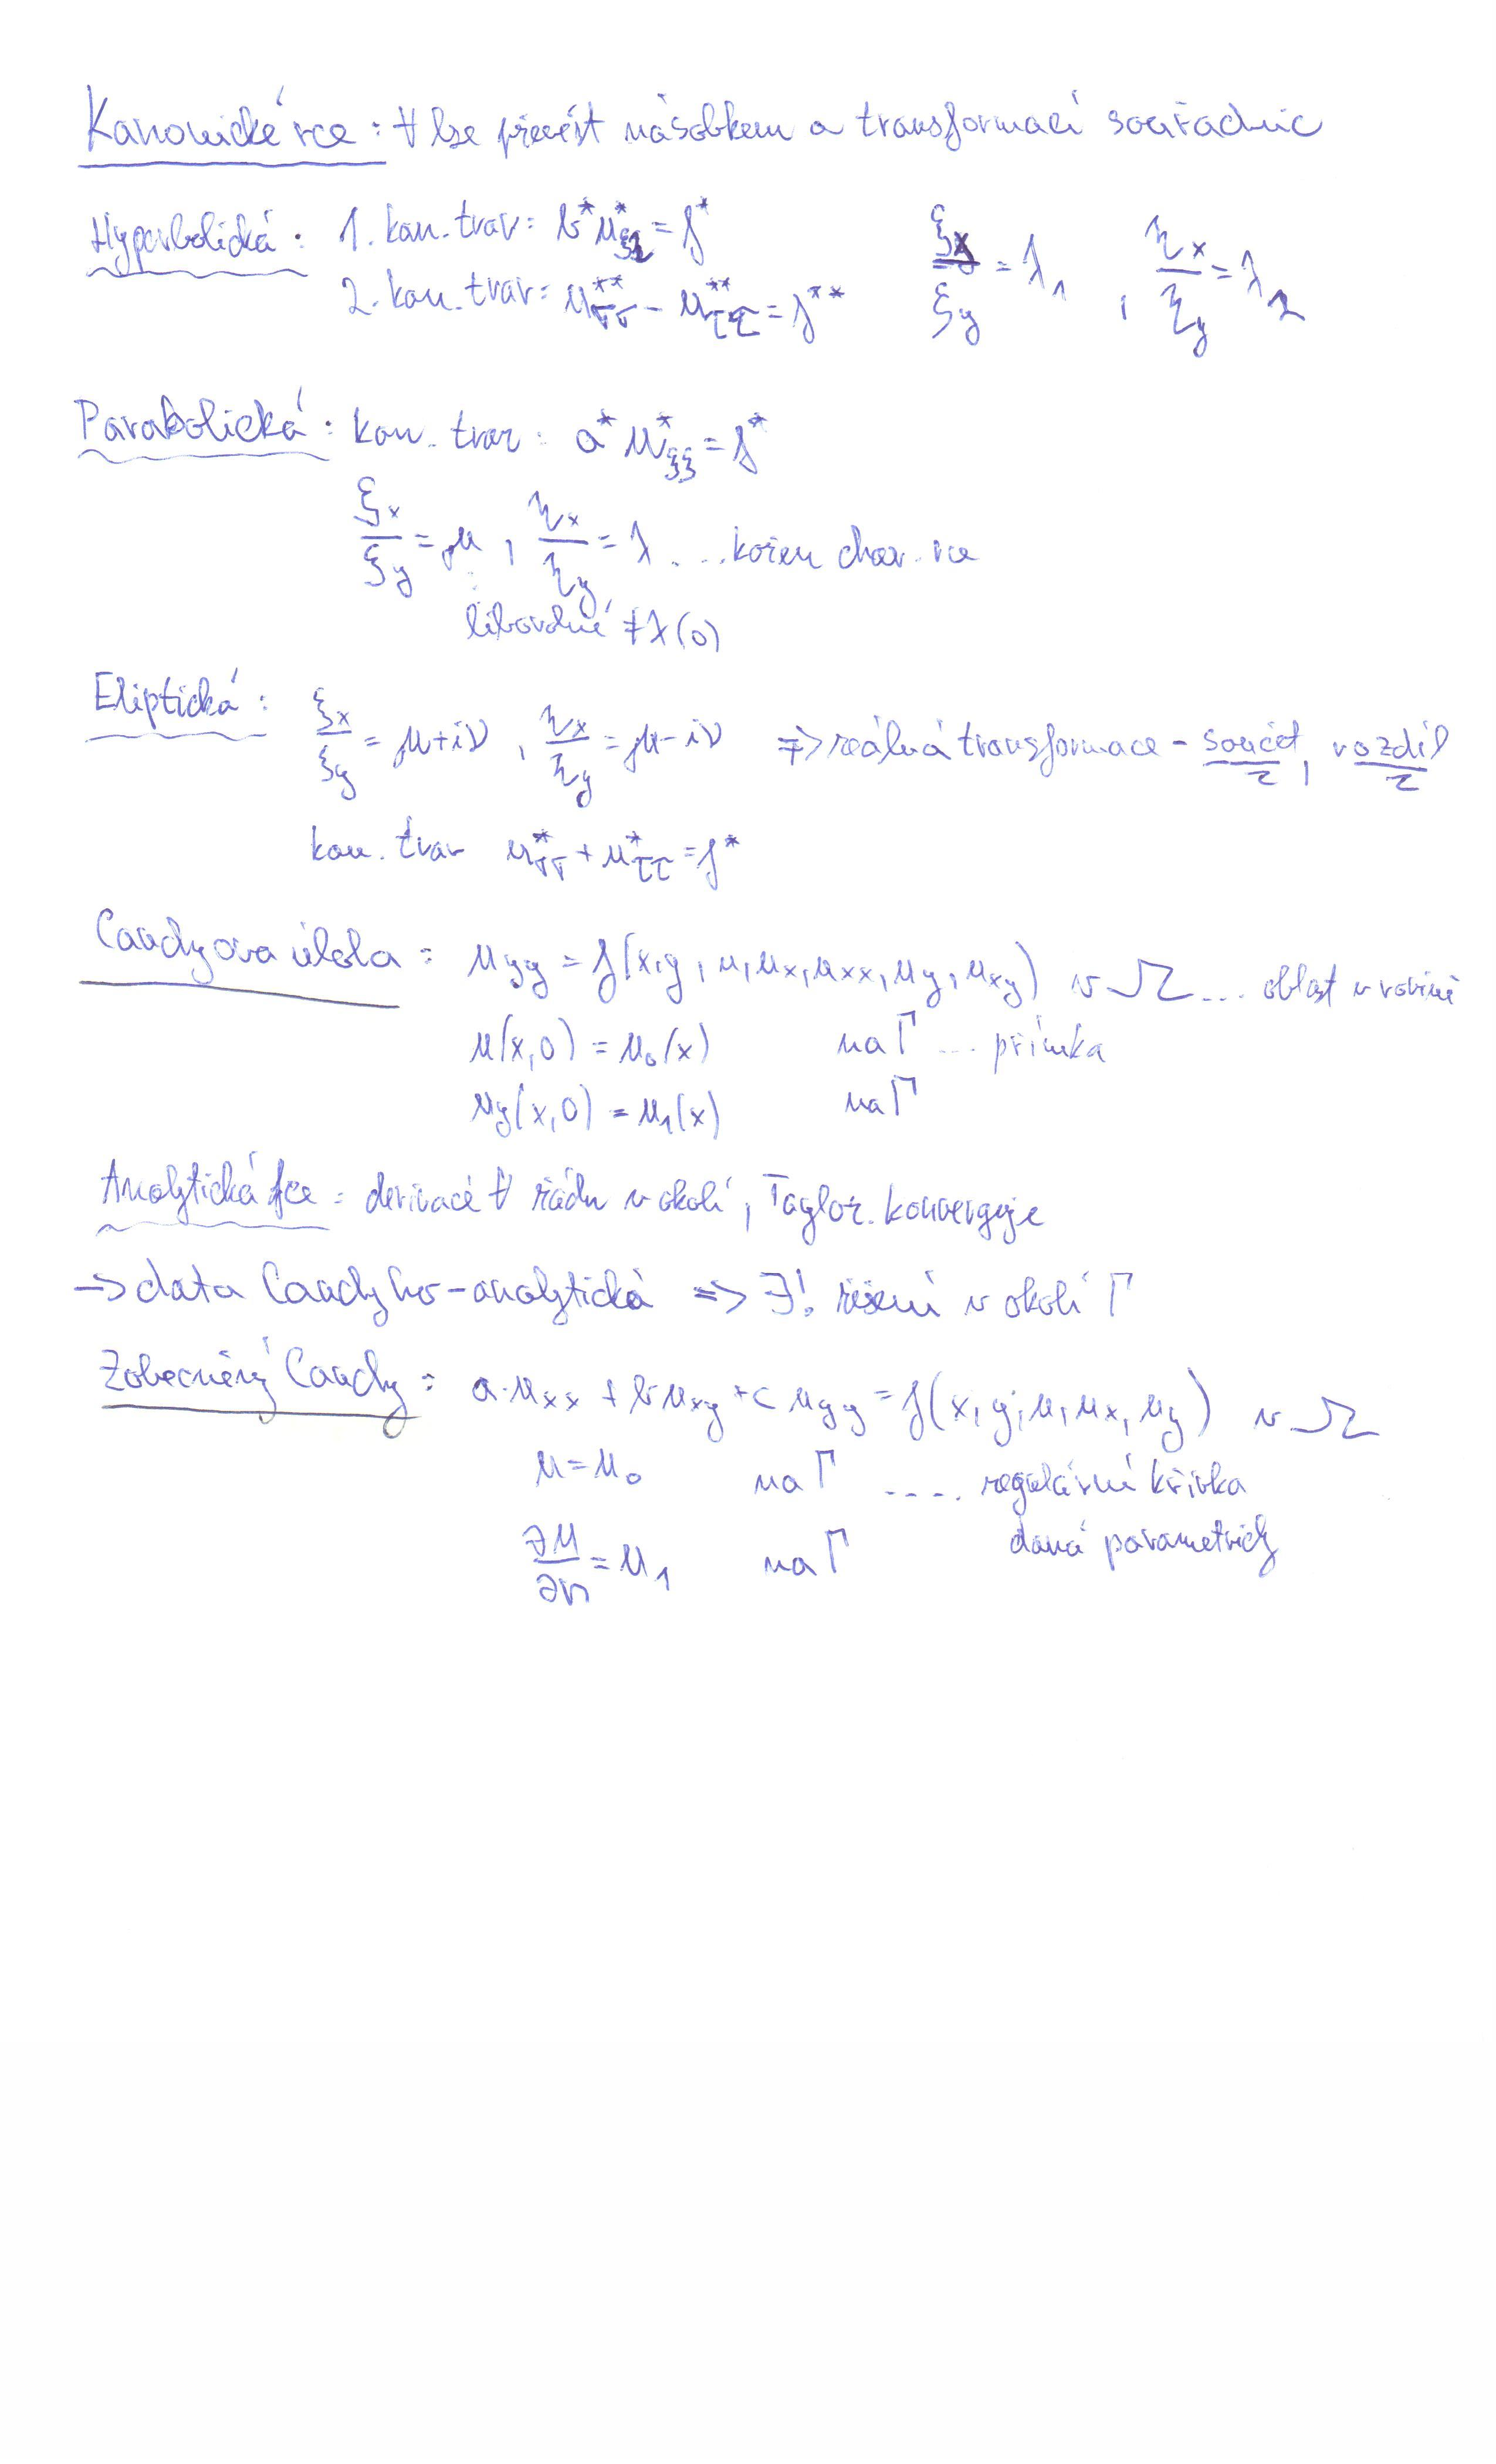
\includegraphics[width=\textwidth]{Obrazky/2-5b.jpg}
\end{figure}

\begin{figure}[H]
\section{Řešení PDR 2}
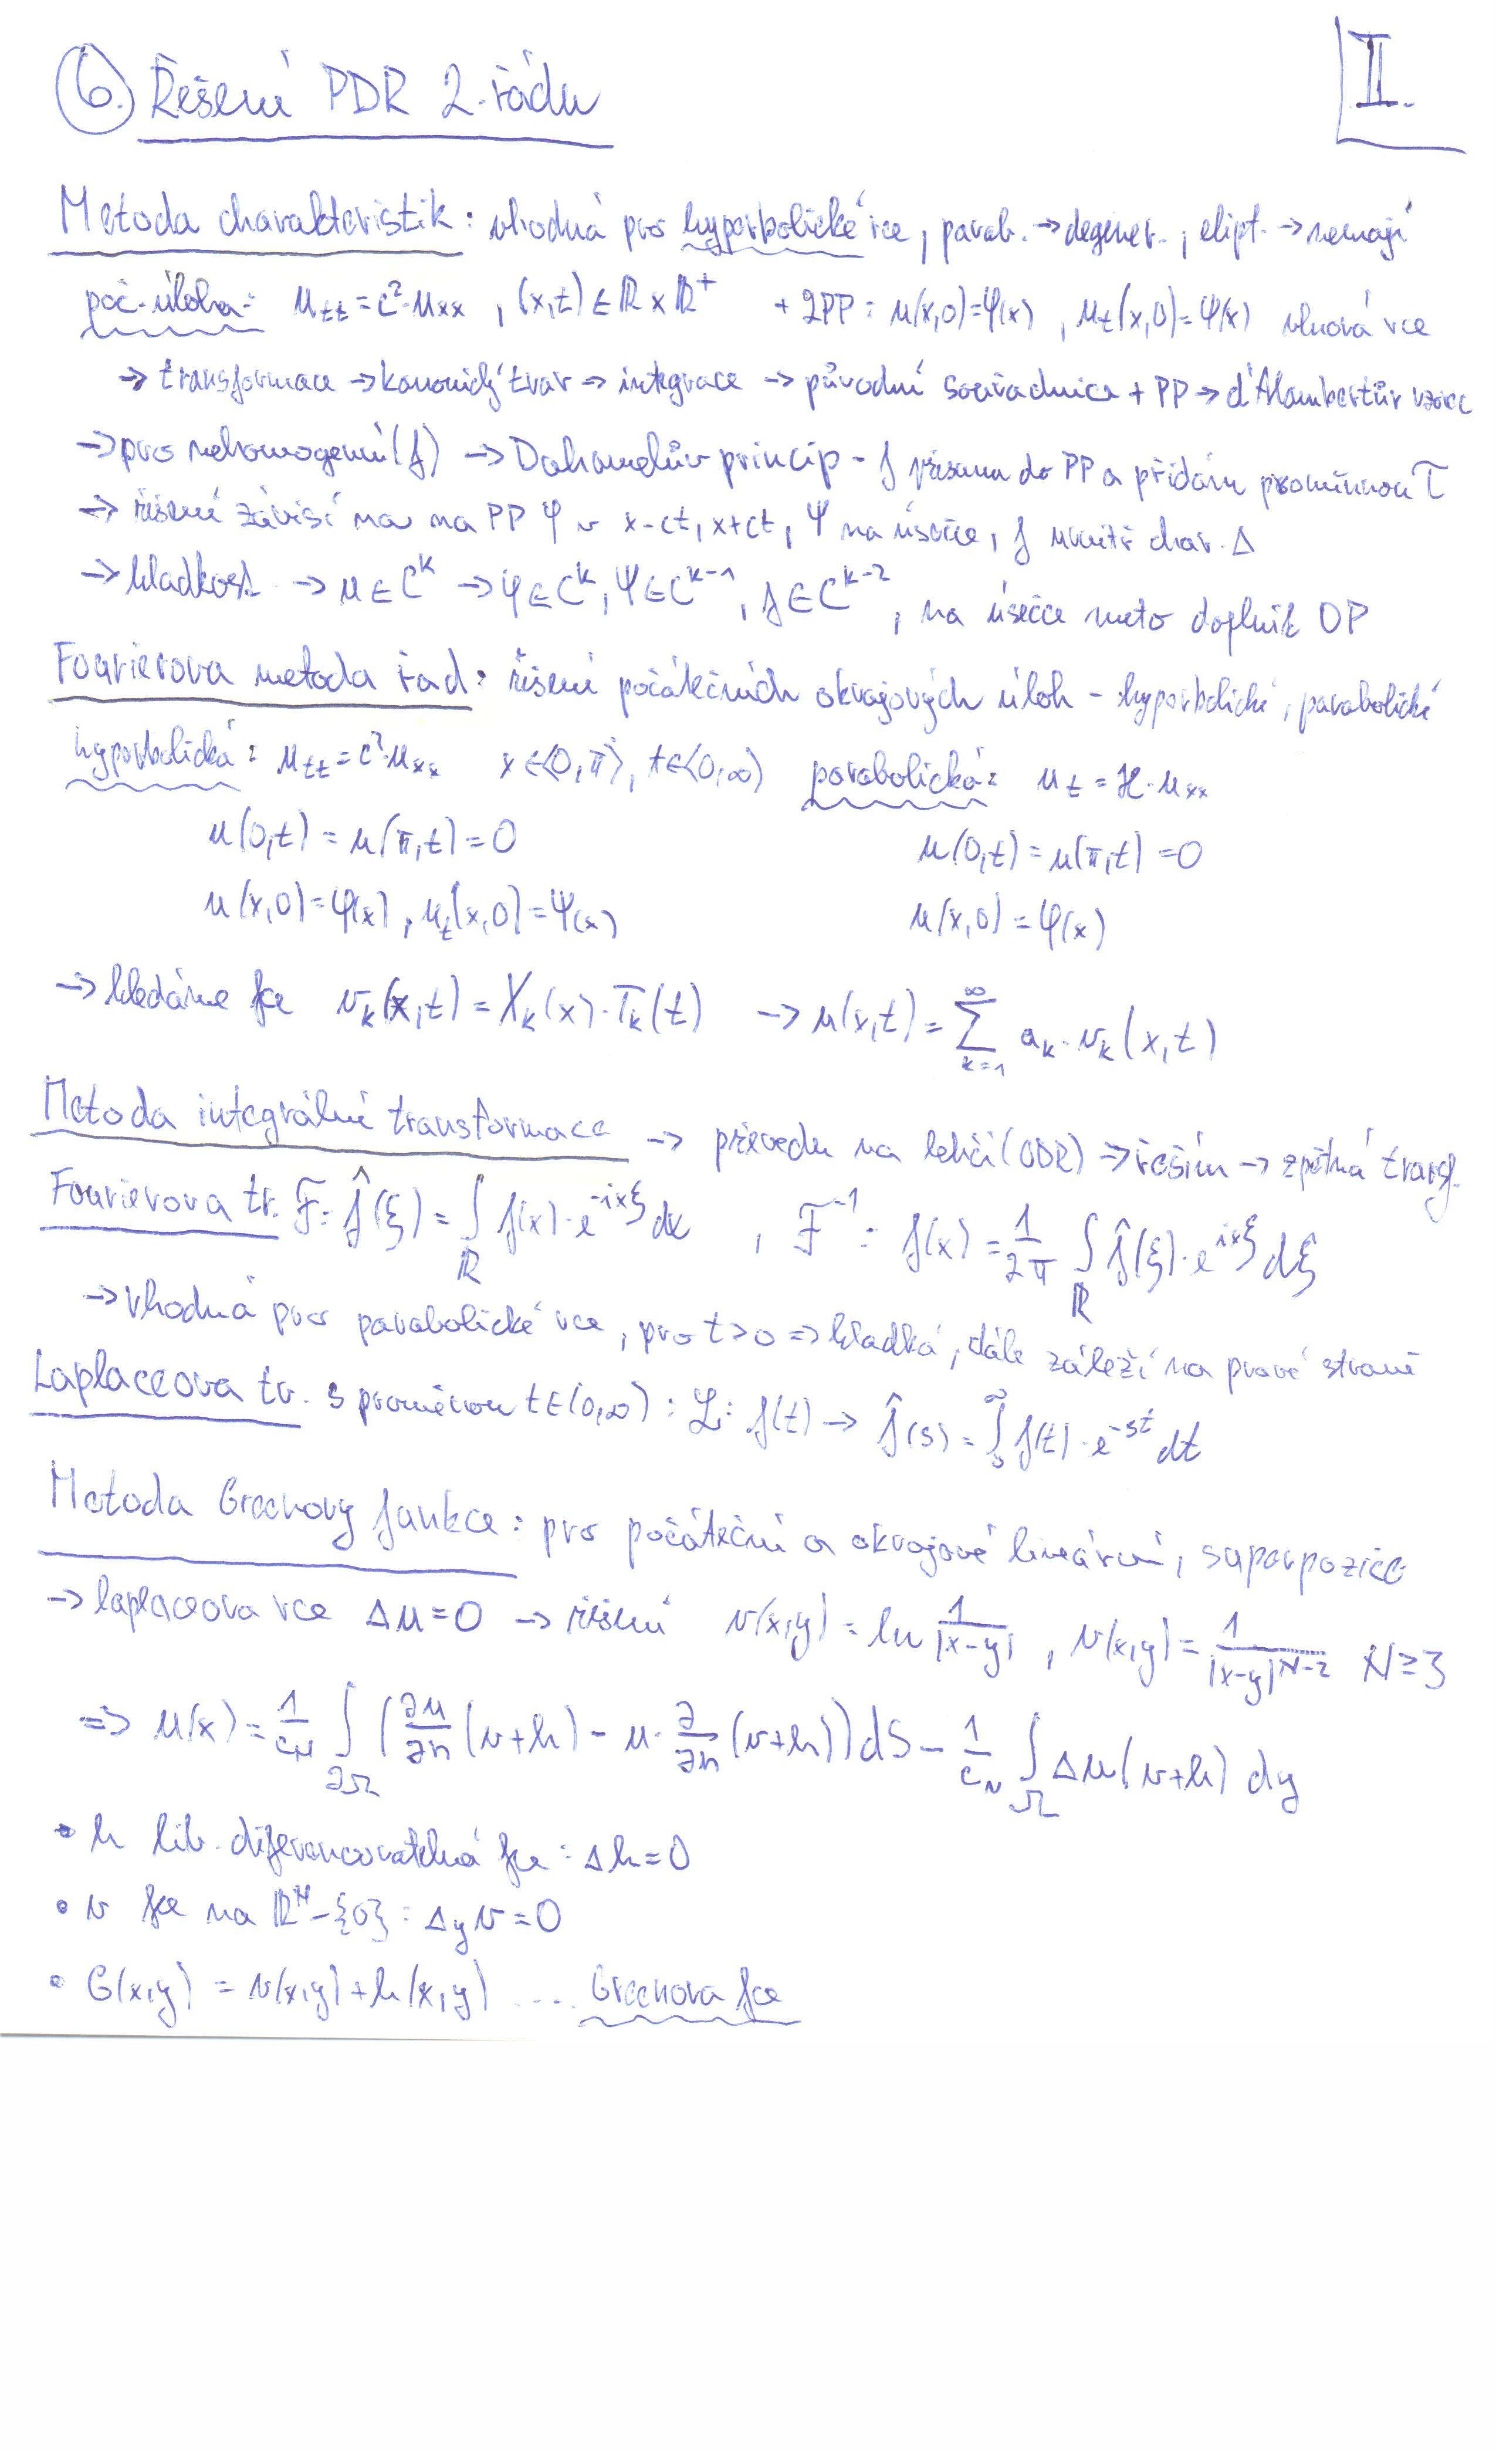
\includegraphics[width=\textwidth]{Obrazky/2-6a.jpg}
\end{figure}

\begin{figure}[H]
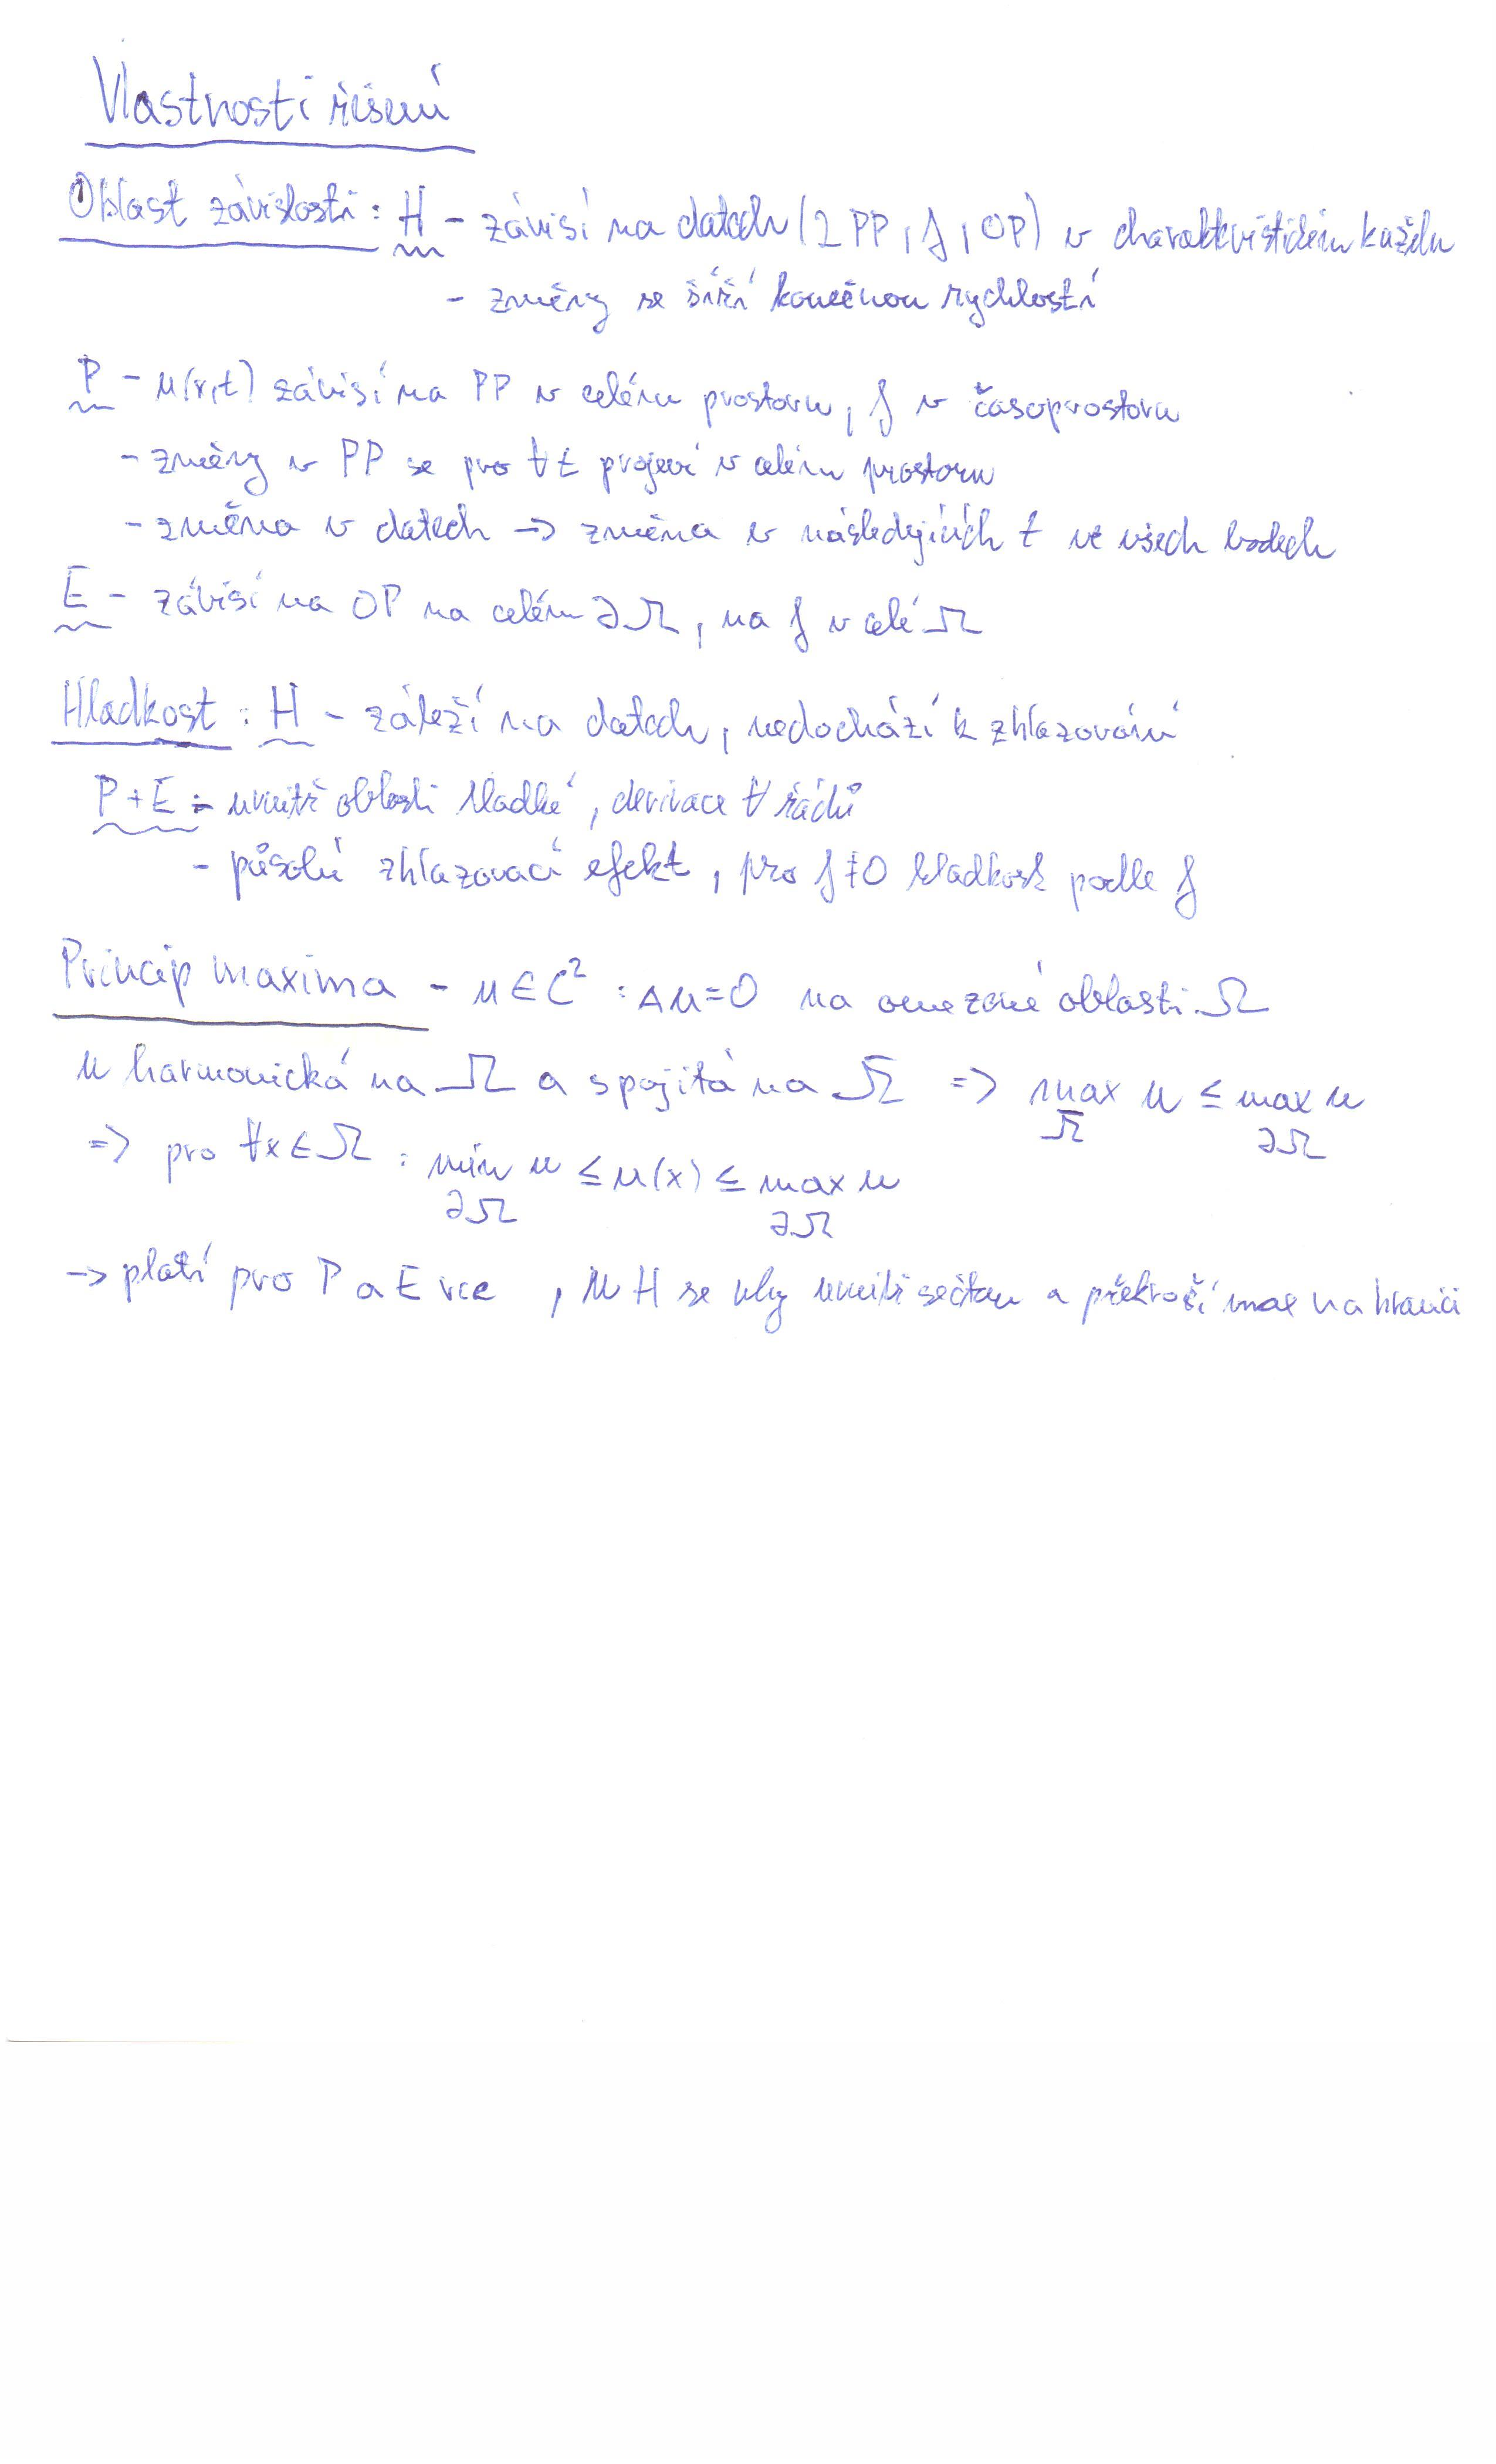
\includegraphics[width=\textwidth]{Obrazky/2-6b.jpg}
\end{figure}


\section{Rovnice matematické fyziky}

\subsection{Přehled}
\begin{itemize}
    \item Parabolická
        \begin{itemize}
            \item $\Omega \subset \mathbb{R}^N$, $I=(t_0,\infty)$
            \item $u_t=\Delta u +f$\ \ \ \ na $\Omega\times I$
            \item (PP) $u(x,t_0)=u_0(x)$\ \ \ \ na $\Omega$
            \item (OP) $\alpha \frac{\partial u}{\partial n} +\beta u=g$\ \ \ \ na $\partial\Omega\times I$
            \item vedení tepla ($u$=teplota, $N=1$ pro tyč, $N=2$ pro desku, $N=3$ pro těleso)
        \end{itemize}
    \item Hyperbolická
        \begin{itemize}
            \item $\Omega \subset \mathbb{R}^N$, $I=(t_0,\infty)$
            \item $u_{tt}=\Delta u +f$\ \ \ \ na $\Omega\times I$
            \item (1.PP) $u(x,t_0)=u_0(x)$\ \ \ \ na $\Omega$
            \item (2.PP) $u_t(x,t_0)=u_1(x)$\ \ \ \ na $\Omega$
            \item (OP) $\alpha \frac{\partial u}{\partial n} +\beta u=g$\ \ \ \ na $\partial\Omega\times I$
            \item kmitání, vlnění ($u$=odchylka, $N=1$ pro příčné, podélné kmity, $N=2$ pro kmitání membrány, bubliny, $N=3$ pro akustické, elektro-magnetické vlny)
        \end{itemize}    
    \item Eliptická
        \begin{itemize}
            \item $\Omega \subset \mathbb{R}^N$
            \item $\Delta u=f$\ \ \ \ na $\Omega$
            \item (PP) $u(x,t_0)=u_0(x)$\ \ \ \ na $\Omega$
            \item (OP) $\alpha \frac{\partial u}{\partial n} +\beta u=g$\ \ \ \ na $\partial\Omega$
            \item ustálený stav předchozích, Poissonova rovnice (při $f=0$ Laplaceova rovnice, vedení elektrického proudu, Airyho funkce napětí,   )
        \end{itemize}  
\end{itemize}

\subsection{Rovnice vedení tepla v tyči}

Nejjednodušším případem vedení tepla je vedení tepla v tenké tyči. Označením tenká tyč myslíme tyč s takovým průřezem, jenž je vzhledem k délce zanedbatelný a v němž jsou všechny uvažované veličiny konstantní.

Zavádíme souřadnici $x$, jenž popisuje tyč podélně a čas $t$. Funkce, která bude v diferenciální rovnici vystupovat jako neznámá, bude $T(x,t)$, což je teplota tyče v okamžiku $t$ a poloze $x$. Předpokládáme, že je tyčka na povrchu izolovaná, abychom mohli zanedbat ztráty teploty do okolí, což ovšem neznamená absolutní oddělení tyčky a okolí (vnější zdroj energie). 

Nyní budeme pracovat s elementem tyčky $(x_a,x_b)$ a elementem času $(t_\alpha, t_\beta)$.

Zavedeme veličinu $Q_a$ (resp. $Q_b$), která říká, jak velké množství tepla vyteče z elementu ven přes konec $x_a$ (resp. $x_b$) během časového intervalu $(t_\alpha,t_\beta)$. Veličina $Q_f$ \mbox{popisuje} množství tepla, které do úseku $(x_a,x_b)$ dodáme během $(t_\alpha,t_\beta)$ zvnějšku (předpo\-kládáme tedy nějaký vnější zdroj tepla působící na tyčku). Dále si rozepíšeme \mbox{jednotlivé} protékající tepla.

\begin{equation}
Q_a =-\int_{t_\alpha}^{t_\beta} q(x_a,t) dt,   
\end{equation}

\begin{equation}
Q_b =\int_{t_\alpha}^{t_\beta} q(x_b,t) dt,   
\end{equation}

\begin{equation}
Q_f =\int_{x_a}^{x_b} \int_{t_\alpha}^{t_\beta} f(x,t) dt dx  ,
\end{equation}

kde funkcí $q(x,t)$ myslíme tepelný tok a funkcí $f(x,t)$ myslíme hustotu výkonu tepelného zdroje.

Uděláme tepelnou bilanci, čimž myslíme souhrn všech tepel, které se v úseku vyskytují. Veličinou $\Delta Q$ myslíme teplo, které po časovém úseku v úseku tyčky zůstalo. Tepelnou bilanci děláme s ohledem na zákon zachování energie. Tuto veličinu si zrovna vyjádříme pomocí funkce $e(x,t)$, která vyjadřuje hustotu vnitřní energie.

\begin{equation}
\Delta Q = Q_f - Q_a -Q_b, 
\end{equation}

\begin{equation}
\Delta Q =\int_{x_a}^{x_b} e(x,t_\beta) dx    -\int_{x_a}^{x_b}  e(x,t_\alpha)dx. 
\end{equation}

Nyní tyto dvě vyjádření $\Delta Q$ dáme do rovnosti a upravíme. Následující úpravy předpokládají potřebné derivace a spojité prostředí.

\begin{equation}
\int_{x_a}^{x_b} e(x,t_\beta)dx-\int_{x_a}^{x_b}  e(x,t_\alpha)dx= \int_{x_a}^{x_b} \int_{t_\alpha}^{t_\beta} f(x,t) dt dx+\int_{t_\alpha}^{t_\beta} q(x_a,t) dt-\int_{t_\alpha}^{t_\beta} q(x_b,t) dt, 
\end{equation}

\begin{equation}
\int_{x_a}^{x_b} \int_{t_\alpha}^{t_\beta} \frac{\partial e}{\partial t} (x,t) dt
dx= \int_{x_a}^{x_b} \int_{t_\alpha}^{t_\beta} f(x,t)-\frac{\partial q}{\partial x} (x,t)dt dx,
\end{equation}

\begin{equation}
\int_{x_a}^{x_b} \int_{t_\alpha}^{t_\beta} \frac{\partial e}{\partial t}(x,t)-f(x,t)+\frac{\partial q}{\partial x} (x,t) dt dx=0 ,
\end{equation}

\begin{equation}
\lim_{x_b\rightarrow x_a} \lim_{t_\beta \rightarrow t_\alpha} \frac{1}{x_b-x_a}\frac{1}{t_\beta-t_\alpha}\int_{x_a}^{x_b} \int_{t_\alpha}^{t_\beta} \frac{\partial e}{\partial t}(x,t)-f(x,t)+\frac{\partial q}{\partial x} (x,t) dt
dx=0 ,
\end{equation}

\begin{equation}    
\frac{\partial e}{\partial t}(x,t)-f(x,t)+\frac{\partial q}{\partial x} (x,t)=0.\label{hxbwkuehbkuwhfcuwkbfwhck} \end{equation}

Doposud bylo odvozování přesné. V dalším přesnost mírně ztratíme z důvodu použití vztahů mezi energií/tepelným tokem a teplotou. 
Dále si funkce výše uvedené upravíme pomocí jiných veličin (konstituční vztahy).
\begin{equation}
e(x,t)=\overline{e}(x,T(x,t))=C(x)T(x,t)+K,
\end{equation}
kde $C(x)$ je množství tepla, které je nutno dodat do jednotkové délky tyče, aby se teplota zvýšila o $1^o C$ (tedy měrná tepelná kapacita neboli měrné teplo), a $K$ je konstanta která při derivování vypadne.
\begin{equation}
\frac{\partial e}{\partial t}=C(x) \frac{\partial T}{\partial t}(x,t)
\end{equation}

Tepelný tok upravíme podle Fourierova zákona vedení tepla (viz podkapitola 2.3) následovně:
\begin{equation}
q(x,t)=-\frac{\partial T}{\partial x}(x,t)\lambda(x),
\end{equation}
kde $\lambda(x)$ je tepelná vodivost a záporné znaménko je tam z důvodu toho, že teplo vždy teče z teplého na studené.

Pokud vše dosadíme do (\ref{hxbwkuehbkuwhfcuwkbfwhck}) dostáváme:

\begin{equation}
C(x) \frac{\partial T}{\partial t}=\frac{\partial }{\partial x} \bigg(\lambda(x)\frac{\partial T}{\partial x}(x,t)\bigg)+f(x,t).
\end{equation}
Dostali jsme tedy parciální diferenciální rovnici druhého řádu.

Měrná tepelná kapacita bývá vztažena většinou na jednotku hmotnosti a nikoli délky. Vztáhneme ji tedy na jednotku hmotnosti úpravou $\rho c(x)=C(x)$, kde $\rho$ je hustota materiálu. Všimněme si, že předpokládáme nezávislost $c(x)$ a $\lambda(x)$ na teplotě. Pokud by hodnoty těchto dvou veličin byly nezávislé i na $x$ a tyčka tedy byla z homogenního materiálu, mohli bychom s nimi zacházet jako s čísly a diferenciální rovnice by vypadala: 

\begin{equation} T^\prime_t=\frac{\lambda}{ c\rho} T^{\prime\prime}_{xx}+\frac{f}{ c\rho}.
\end{equation}

K jednoznačnému řešení úlohy vedení tepla v tyči ovšem ještě potřebujeme počáteční podmínku v čase $t_0$ (v případě tyčky konečné délky následující platí pro $x\in (a,b)$ a v případě tyče nekonečné délky $x\in \mathbb{R}$).
\begin{equation} 
T(x,t_0)=T_0 (x).
\end{equation}

To by stačilo v případě nekonečně dlouhé tyče. V případě tyče konečné délky je ještě potřeba dodat okrajové podmínky, které mohou být vícero druhu. První uvedeme Dirichletovy podmínky, které říkají, jaká teplota je na okrajích tyčky.
\begin{equation}
T(x_a,t)=T_a(t), \ \ \ \ \ 
T(x_b,t)=T_b(t),  \ \ \ \ \   t>t_0.
\end{equation}
Dalším typem okrajových podmínek jsou Neumannovy okrajové podmínky, které předepisují tepelný tok na okrajích.
\begin{equation}
T^\prime_x(x_a,t)=g_a(t),  \ \ \ \ \
T^\prime_x(x_b,t)=g_b(t), \ \ \ \ \      t>t_0.
\end{equation}
Posledním typem jsou Robinovy okrajové podmínky, které jsou kombinací prvních dvou. V následujícím musí být $\alpha$ a $\beta$ větší než nula, protože jinak by se jednalo \mbox{o předchozí} podmínky.
\begin{equation}
-\alpha_a T^\prime_x(x_a,t)+\beta_a T(x_a,t)=g_a(t), \ \ \ \ \
\alpha_b T^\prime_x(x_b,t)+\beta_b T(x_b,t)=g_b(t),\ \ \ \ \   t>t_0.
\end{equation}

Diferenciální rovnice popsaná v předešlém je \textbf{parabolického} typu.

\subsection{Rovnice vedení tepla v tělese}
Tuto rovnici zde uvedeme bez odvození a pouze s popisem okrajových podmínek a jednoho konstitučního vztahu týkajícího se Fourierova zákona. Teplota je značena jako $T(x_1,x_2,t)$. Měrná tepelná kapacita je značena jako $c(x_1,x_2)$. Tepelný tok je značen jako $\mathbf{\dot{q}}(x_1,x_2)$. Hustota materiálu je $\rho (x_1,x_2)$ a hustota vnitřního zdroje je značena $f(x_1,x_2)$.

\begin{equation}
c \rho T_t^\prime+div(\mathbf{\dot{q}})-f=0 .
\end{equation}

Úprava tepelného toku lze rozdělit na více případů zavisejících na druhu materiálu.
\begin{itemize}
\item Izotropní materiál:
$\dot{q}_i=-\lambda\frac{\partial T}{\partial x_i}$, kde $\lambda$ je tepelná vodivost.
\item Anizotropní materiál v hlavních směrech:\\
$\dot{q}_i=-\lambda_i \frac{\partial T}{\partial x_i}$, kde $\lambda_i$ je tepelná vodivost ve směru $i$.
\item Anizotropní materiál obecně:\\
$\dot{q}_i=-\sum_{j=1}^{3} \lambda_{ij}\frac{\partial T}{\partial x_j}$, kde $\lambda_{ij}$ je symetrická matice tepelných vodivostí.
\end{itemize}

Uvedeme zde nyní parciální diferenciální rovnici popisující vedení tepla v izotropním tělese.
\begin{equation}
c \rho T_t^\prime=\lambda\Delta T +f\ .
\label{diferencialnirovnicepopisujicivednitepla}    
\end{equation}
 Opět je nutné uvést počáteční a případně i okrajové podmínky. Pokud se úloha týká celého prostoru, potom $\Omega = \mathbb{R}^3$:
\begin{equation}
T(\mathbf{x},t_0)=T_0(\mathbf{x}),\ \ \ \mathbf{x}\in\Omega,\ t>t_0.
\label{pocatecnipodminkapopisujicivednitepla}   
\end{equation}
Pokud je těleso konečných rozměrů, tak je potřeba dodat okrajové podmínky, \mbox{kterých} je opět vícero druhů:
\begin{itemize}

\item Dirichletovy OP: $T(\mathbf{x},t)=T_0(\mathbf{x},t), \ \ \ \ \mathbf{x}\in \partial\Omega $
\item Neumannovy OP: $ \frac{\partial T}{\partial n}(\mathbf{x},t)=g(\mathbf{x},t),  \ \ \ \ \mathbf{x}\in \partial\Omega      $

\item Robinovy OP: $ \frac{\partial T}{\partial n}(\mathbf{x},t)=-k_0 [T(\mathbf{x},t)-g(\mathbf{x},t) ],\ \ \ \ \mathbf{x}\in\partial\Omega$

\end{itemize}

Počáteční problém pro těleso s konečnými rozměry je tedy dán (\ref{diferencialnirovnicepopisujicivednitepla}), (\ref{pocatecnipodminkapopisujicivednitepla}) a některou z okrajových podmínek.

Diferenciální rovnice popsaná v předešlém je \textbf{parabolického} typu.

\subsection{Rovnice kmitání struny}
 Provedeme silovou bilanci úseku struny $(x_a,x_b)$ v čase $t$. Neznámou funkcí je $u(x,t)$, což značí kolmou výchylku struny v čase $t$ a místě $x$. Síla, kterou je struna napjatá, je $T$. Uvažujeme pohyb ve směru osy $y$. Pohyb ve směru osy $x$ zanedbáme. Předpokládáme tenkou strunu, v čemž se skrývá zanedbání odporu struny vůči ohýbání. Kmity předpokládáme "malé" a proto zanedbáme rozdíl mezi $sin \ \alpha$ a $tg \ \alpha$.
 
 Pro úsek struny $(x_a,x_b)$ v čase $t$ provedeme bilanci průmětů do osy $y$ sil působících na tento úsek.
 $$F_a, F_b=\textrm{průměty sil, kterými působí zbytek struny na úsek v jeho koncích }x_a,x_b $$
 $$F_f=\textrm{průměty známé vnější síly, například gravitace }$$
 
 Hlavní myšlenkou silové bilance bude Newtonův zákon. Výslednice sil působících na strunu je součinem hmotnosti a zrychlení. Jako celkovou sílu působící na úsek budeme označovat $F$. Funkce $f(x,t)$ charakterizuje vliv zdroje v místě $x$ a čase $t$. Úhel, který svírá struna a osa $x$, je značen v bodě $x_a$ jako $\alpha$ a v bodě $x_b$ jako $\beta$.

\begin{equation}
F_f=\int_{x_a}^{x_b} f(x,t)\ dx
\end{equation}
\begin{equation}
F_b=T sin \ \beta \doteq T tg\ \beta=T u_x (x_b,t)
\end{equation}
\begin{equation}
F_a=-T sin \ \alpha \doteq -T tg\ \alpha=-T u_x (x_a,t)
\end{equation}
\begin{equation}
F=\int_{x_a}^{x_b} \rho u_{tt}(x,t)\ dx
\end{equation}
\begin{equation}
F_a+F_b+F_f=\int_{x_a}^{x_b}f(x,t)\ dx+T\bigg(u_x(x_b,t)-u_x(x_a,t)\bigg)
\end{equation}
\begin{equation}
u_x(x_b,t)-u_x(x_a,t)=\int_{x_a}^{x_b} \frac{\partial }{\partial x} u_x \ dx
\end{equation}
\begin{equation}
F=F_f+F_a+F_b
\end{equation}
\begin{equation}
\int_{x_a}^{x_b} \rho u_{tt}(x,t)\ dx=\int_{x_a}^{x_b} \bigg( Tu_{xx}(x,t)+f(x,t)\bigg)\ dx
\end{equation}
\begin{equation}
lim_{x_b \rightarrow x_a} \frac{1}{x_b-x_a} \int_{x_a}^{x_b} \rho u_{tt}(x,t)\ dx=\rho u_{tt}(x,t)
\end{equation}
\begin{equation}
lim_{x_b \rightarrow x_a} \frac{1}{x_b-x_a} \int_{x_a}^{x_b} \bigg( Tu_{xx}(x,t)+f(x,t) \bigg)\  dx=Tu_{xx}(x,t)+f(x,t)
\end{equation}
\begin{equation}
\rho u_{tt}=Tu_{xx}+f
\label{konecnadiferencialnirovukmitanistruny}
\end{equation}
 
 Rovnice \ref{konecnadiferencialnirovukmitanistruny} je tedy diferenciální rovnicí popisující kmitání struny (pro malé $u_x$). Dále si uvedeme možné počáteční úlohy a okrajové podmínky.
 
 Typy okrajových podmínek:
 \begin{itemize}
 \item Dirichletova: $u(b,t)=u_b(t)$, tzn. předepsaná výchylka struny na koncích.
 \item Neumannova: $u_x(b,t)=g_b(t)$ tzn. zadaná síla na koncích.
 \item Robinova (Newtonova): $u_x(b,t)+ku(b,t)=g_b(t)$, tzn. síla závisí od výchylky.
 \end{itemize}

 Počáteční úloha pro nekonečnou strunu:
 \begin{itemize}
 \item $\rho u_{tt}=Tu_{xx}+f, \ \ x\in(-\infty,\infty), \ t\in(0,\infty) \ \ \ \textrm{(R)}$
 \item $u(x,0)=\phi(x)), \ \ x\in(-\infty,\infty) \ \ \ \textrm{(1.PP)}$
 \item $u_t (x,0)=\psi(x), \ \ x\in(-\infty,\infty)  \ \ \ \textrm{(2.PP)}$
 \end{itemize}
 
 Počáteční okrajová úloha pro úsek struny $(0,L)$:
 \begin{itemize}
 \item $ \rho u_{tt}=Tu_{xx}+f, \ \ x\in(0,L),\ t\in(0,\infty)  \ \ \ \textrm{(R)}$
 \item  $ u(x,0)=\phi(x)), \ \ x\in(0,L) \ \ \ \textrm{(1.PP)}$
 \item  $ u_t (x,0)=\psi(x), \ \ x\in(0,L)  \ \ \ \textrm{(2.PP)}$
 \item $\textrm{Dirichlet, Neumann Robin} \ \ \ \textrm{(OP)} $
 \end{itemize}
 
 Diferenciální rovnice popsaná v předešlém je \textbf{hyperbolického} typu.
%\begin{figure}[h!]
%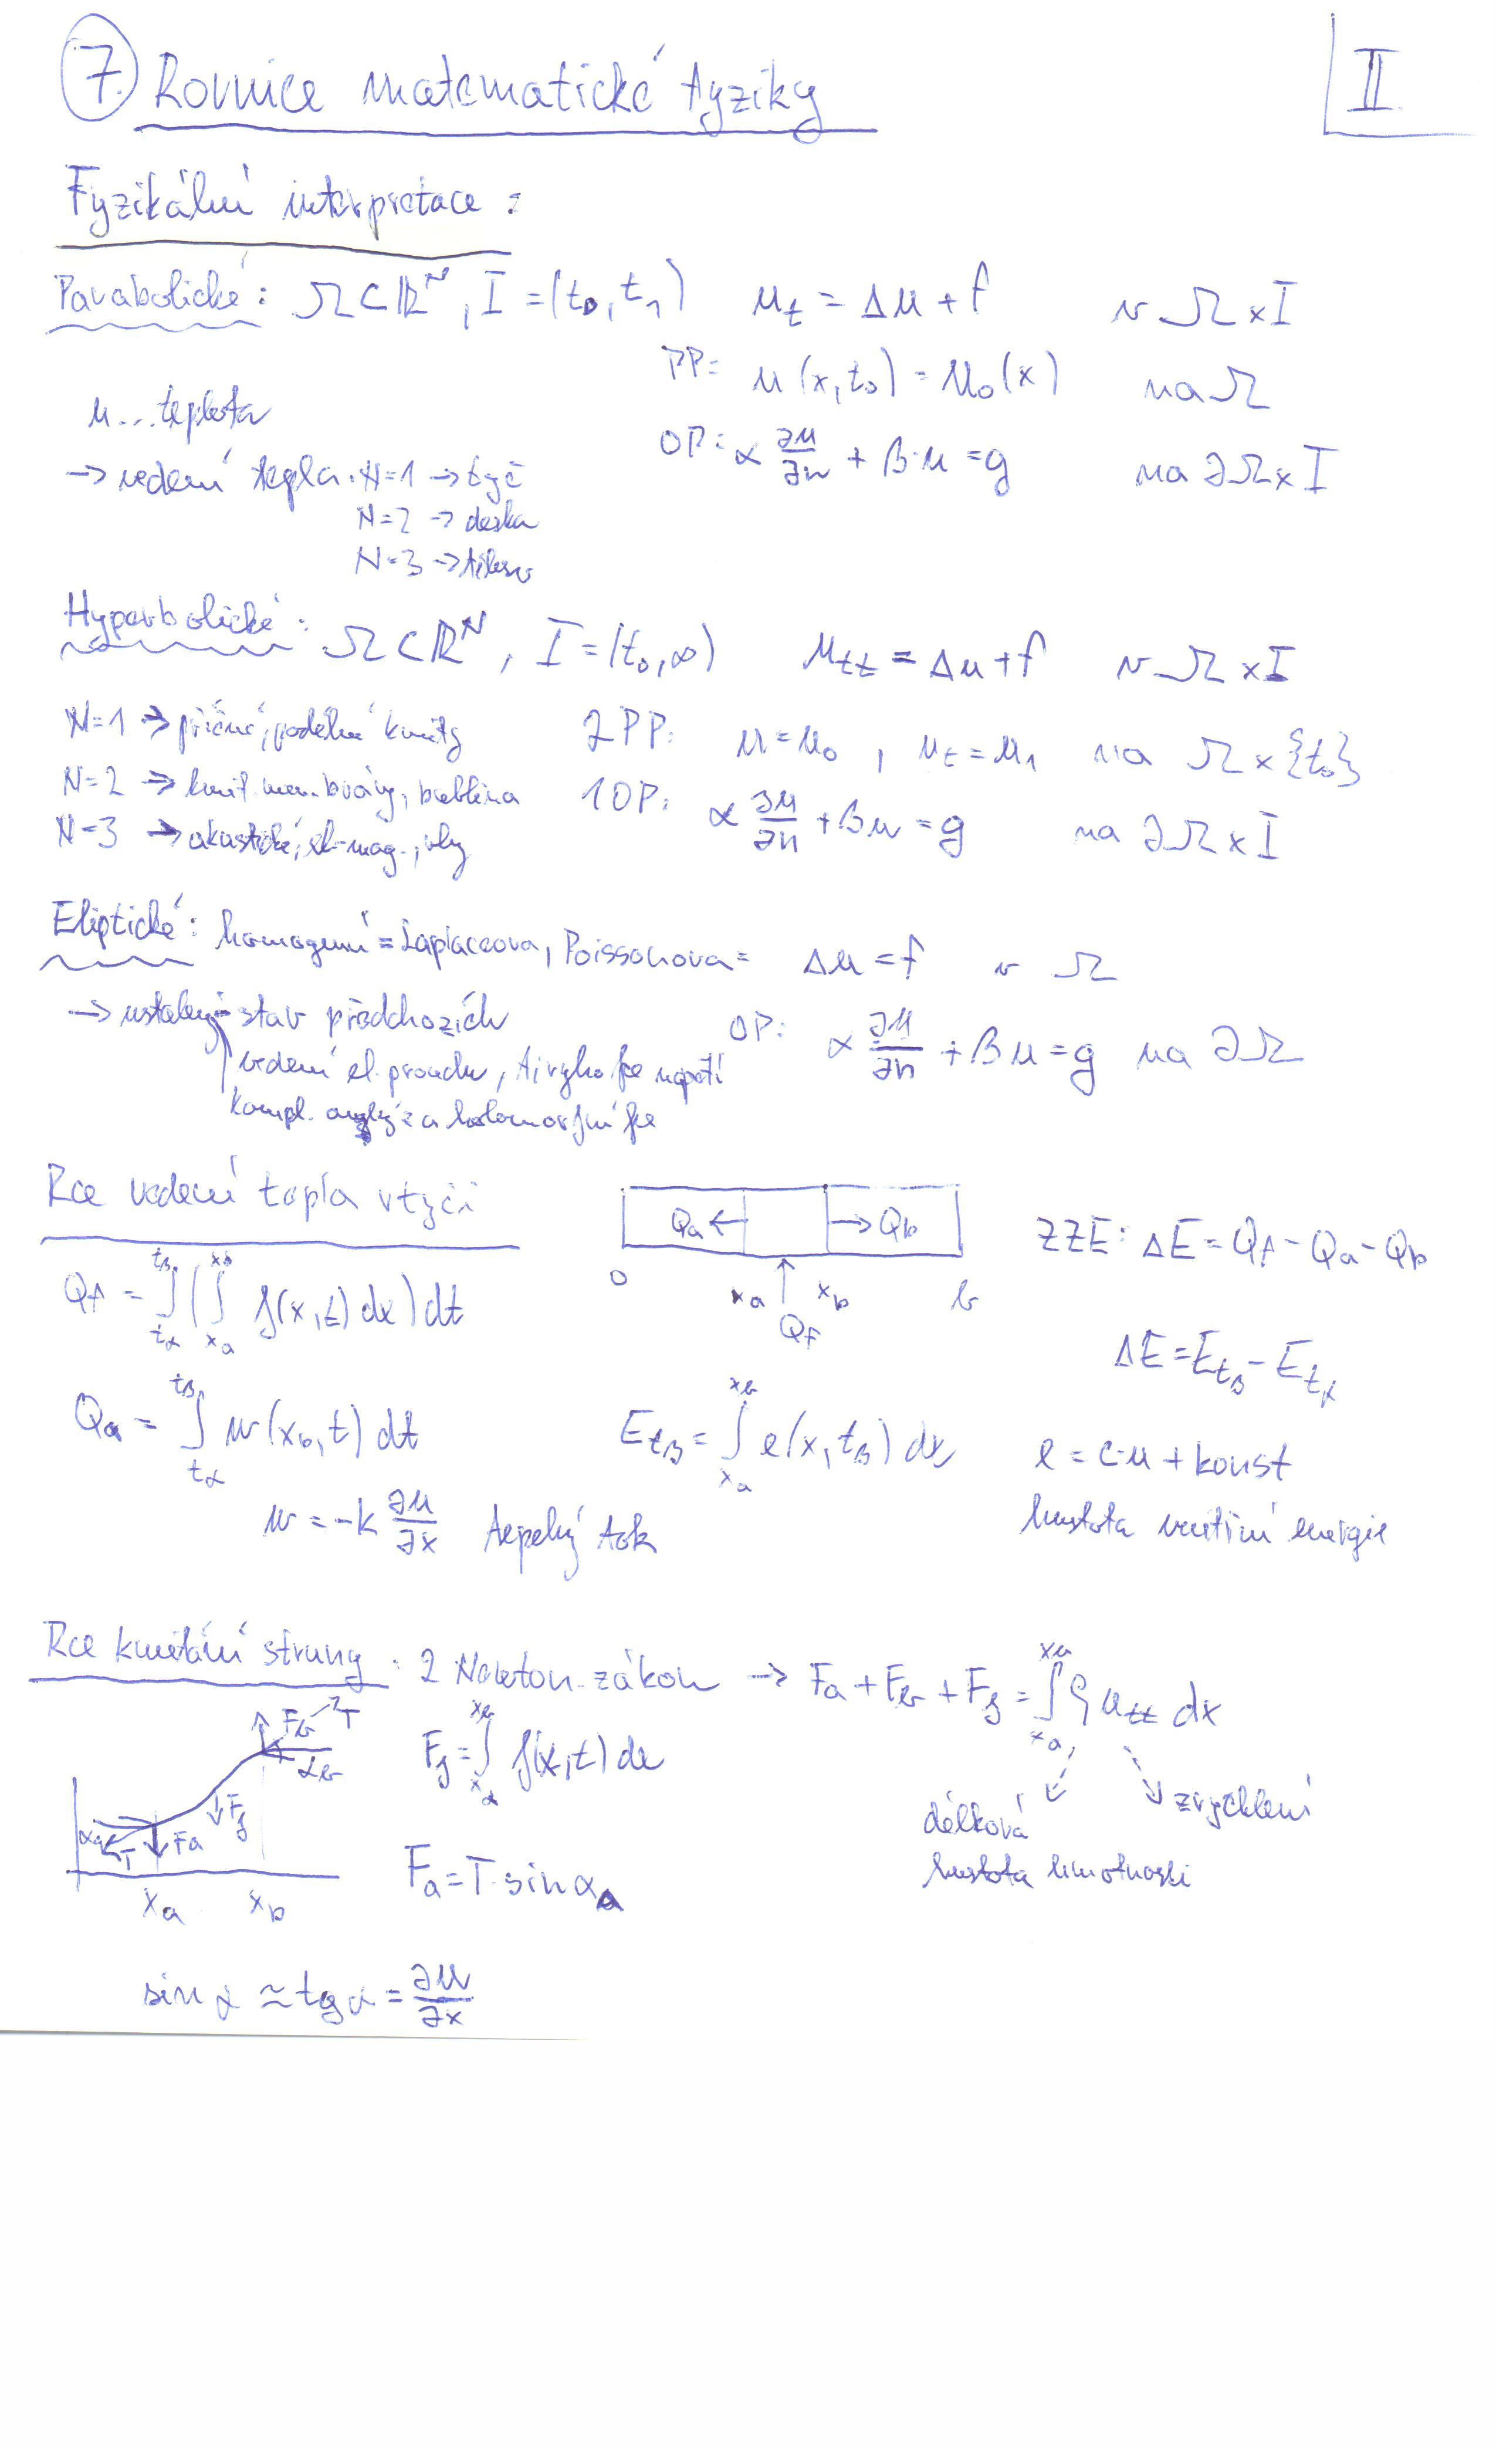
\includegraphics[width=\textwidth]{2-7a.jpg}
%\end{figure}
%\begin{figure}[h!]
%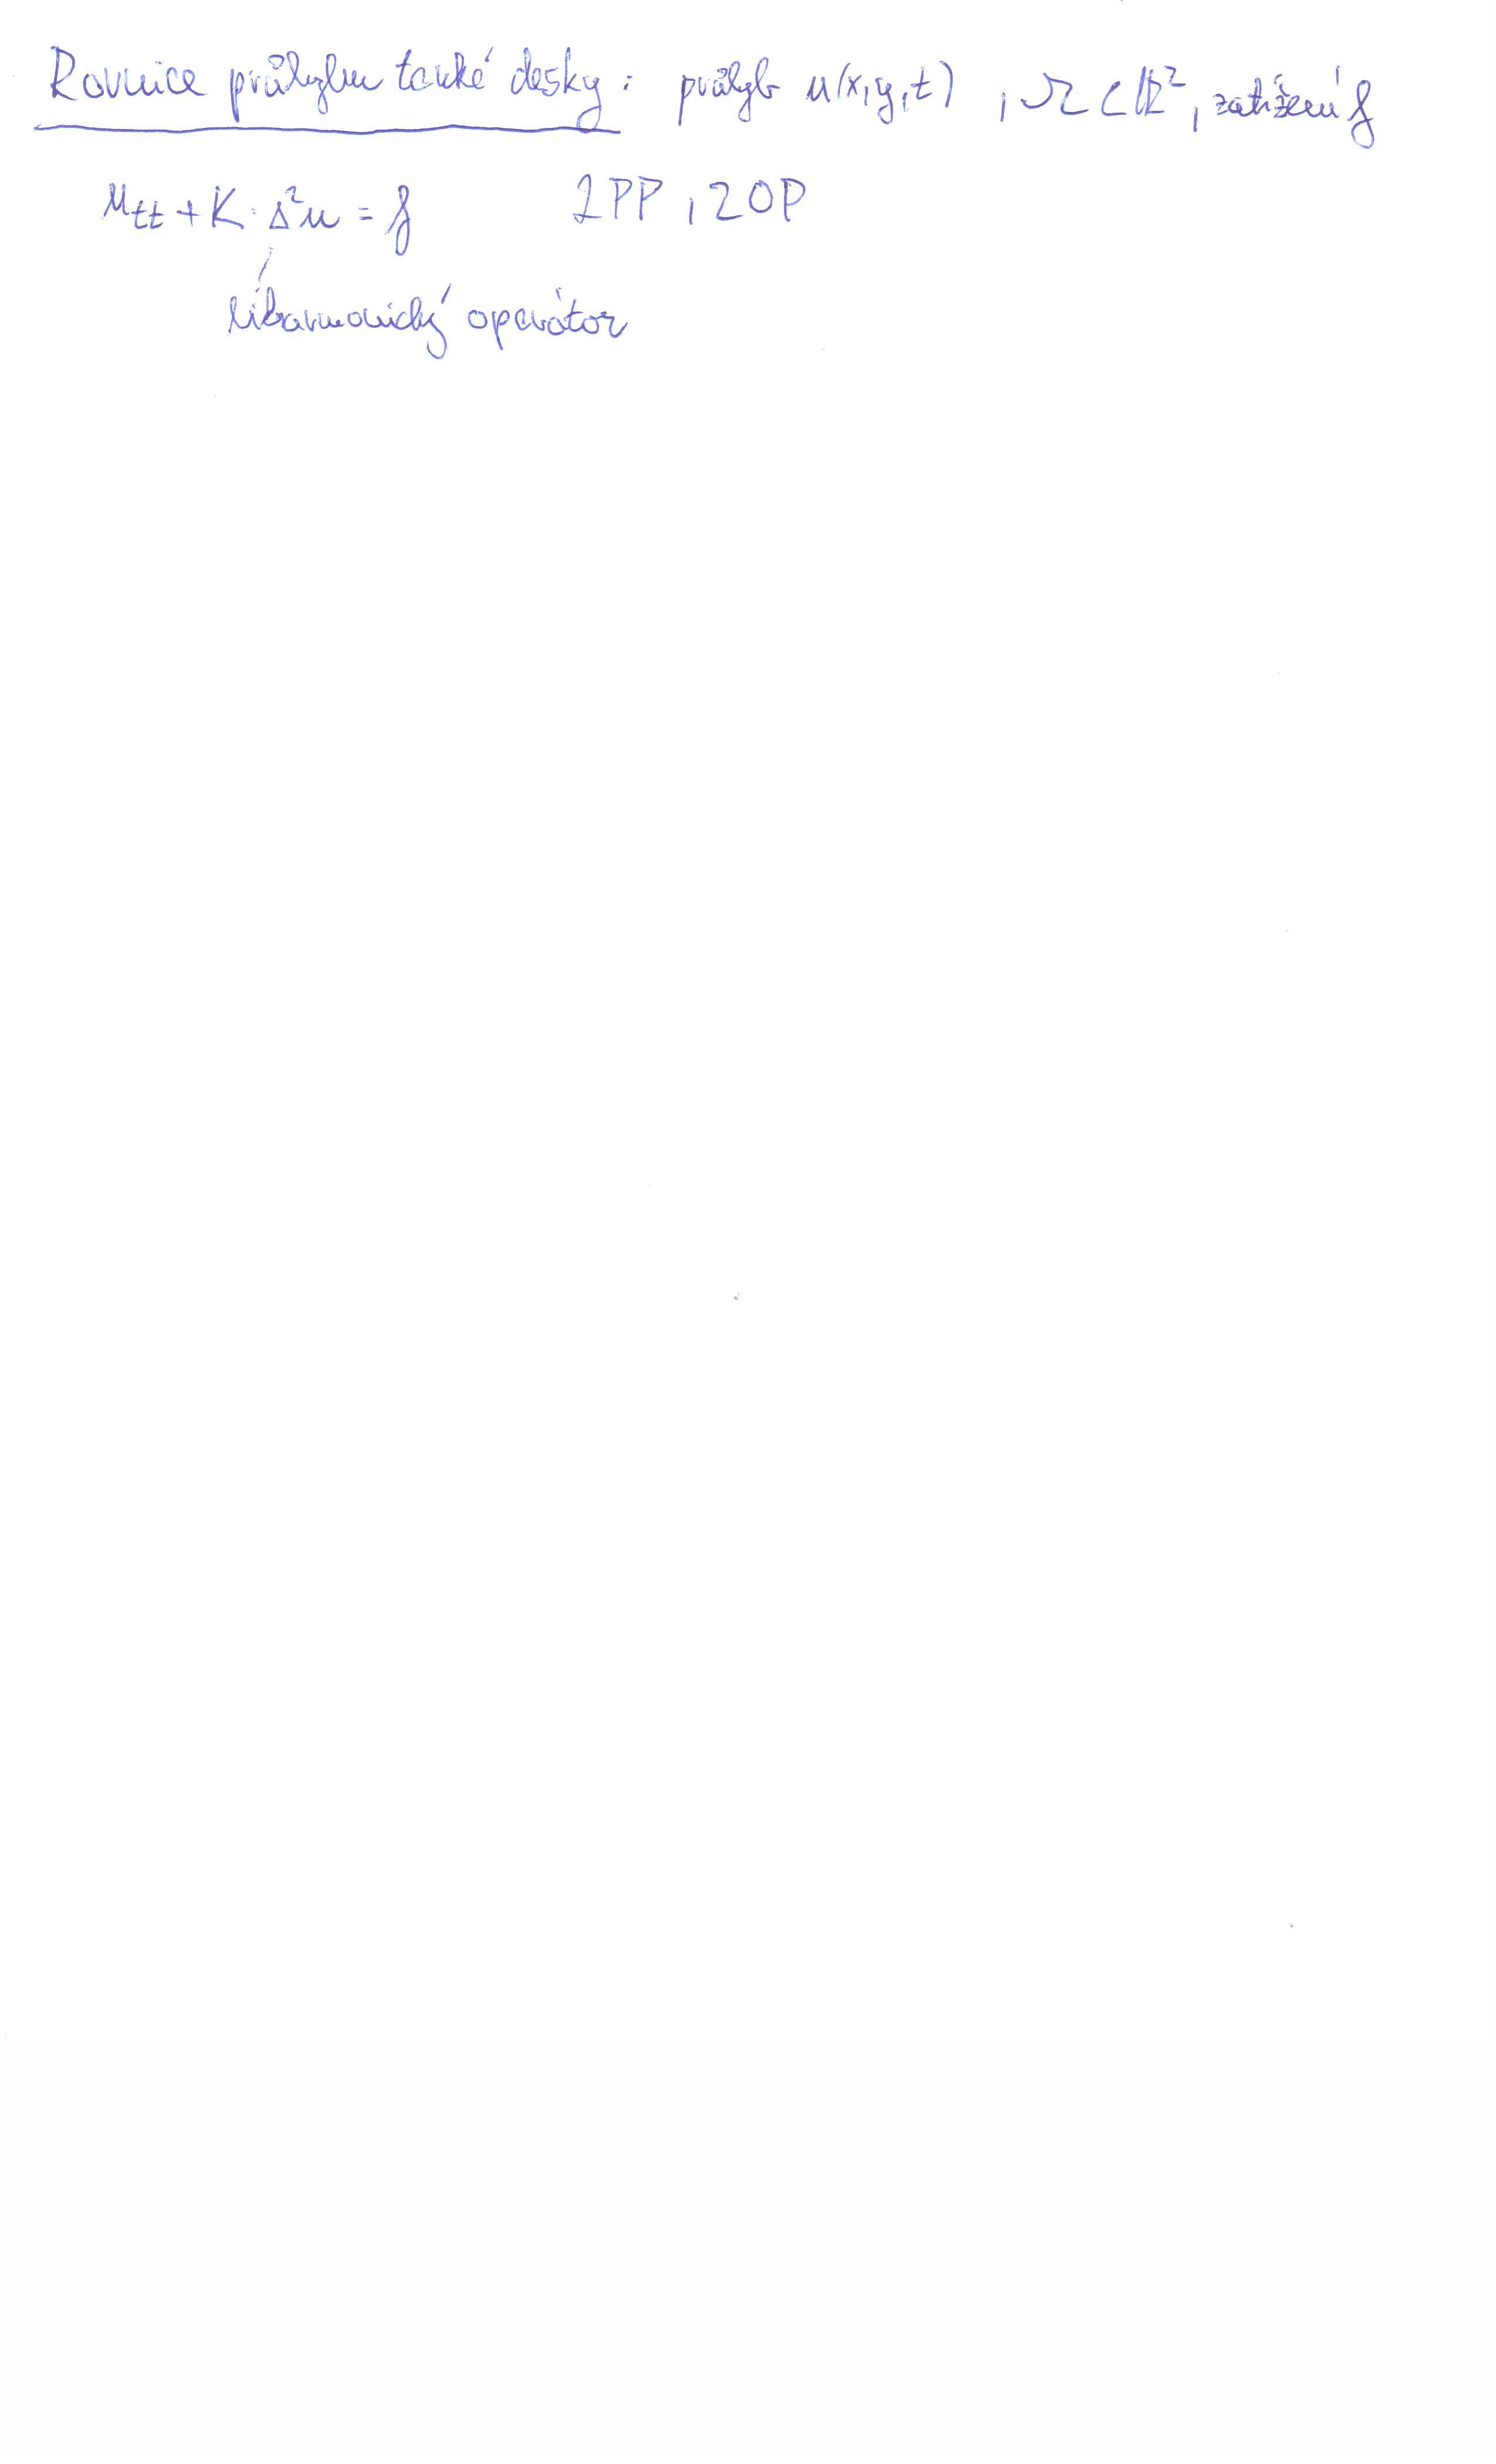
\includegraphics[width=\textwidth]{2-7b.jpg}
%\end{figure}



\section{Moderní řešení PDR}

\section{Konečnorozmérné aproximace PDR}

\section{Diferenciální geometrie}
